%========================================================================
%\newcommand*\dsk{/home/danaila/A_COMMON/RECHERCHE}
%\newcommand*\dsk{D:/A_COMMON/RECHERCHE}

\newcommand*\dsk{./}

\newcommand*\figpath{\dsk/A_figs}
\newcommand*\bibpath{\dsk/A_bib}
\newcommand*\stypath{\dsk/A_style}
\newcommand*\incpath{.}
%========================================================================

%========================================================================
%\documentclass[twoside,fontsize=11pt,headsepline,french]{scrbook}
\documentclass[twoside,fontsize=12pt,headsepline,english]{scrbook}
%========================================================================

%========================================================================

\usepackage{graphicx}   %% envir graphique pour latex ou pdflatex
%\usepackage[T1]{fontenc}     %% pour la cesure avec les accents
\usepackage[latin1]{inputenc} %% problemes d'accents
\usepackage[colorlinks=true, linkcolor=myred, citecolor=myred]{hyperref}         %% links dans le dvi

\usepackage{amsmath,amsfonts,amssymb}
\usepackage{mathrsfs}
\usepackage{amsthm}
\usepackage{pdfpages}	% % introduire plusieurs pages pdf
\usepackage{booktabs}	% % Tableau style

%\usepackage[sectionbib,gather]{chapterbib}       %%  pour la biblio locale (projet)
\usepackage{times}            %% pour pdf avec de jolie police
\usepackage{colordvi}        %% couleurs dans le dvi
%\usepackage[monochrome]{color}
\usepackage{color}
\usepackage{xcolor}
%\usepackage{amssymb,epic}
%\usepackage[french]{minitoc}   % mini-sommaires pour chaque chapitre
\usepackage{multimedia}       %% pour les films
\usepackage{array,multirow,makecell}  % pour fusionner les cellules dans un tableau
%========================================================================
%\usepackage[english]{babel}
%\usepackage[frenchb]{babel}    %% style french
%------------------------------%% titres en francais
%\addto\captionsfrench{\renewcommand{\figurename}{\em Figure}%
%\renewcommand{\tablename}{\em Tableau}%
%\renewcommand{\chaptername}{\em }
%\renewcommand{\summaryname}{Sommaire}}
%========================================================================
%\usepackage{\stypath//floatflt}         %% figures dans les paragraphes -- il est nul
%=======================================biblio en anglais(non compat avec cite)
\usepackage[round]{natbib}
%\usepackage[]{natbib} 

%\bibliographystyle{plainnat}
%                     \cite{}     %citation normale
%                     \citet{}    %textuel
%                     \cite[texte avant][texte apres]{}
%                     \citep{}    %avec parenth{\`e}ses
%                     \citealt{}, \citealp{}    %sans aucune parenth{\`e}se
%                      \citeyear{},\citeauthor{}
%
%=======================================biblio en francais
%\bibliographystyle{\stypath//plainnat-io}
%\bibliographystyle{abbrvnat-fr} % biblio style francais
%\usepackage{\stypath//frbib}
%\bibliographystyle{\stypath//frcomplet}
%%%%%%%%%%========================================================================
%   --- couleurs
\definecolor{myred}{rgb}{0.8,0.1,0.1}

\def\textRed{\color{red}}
\def\textBlack{\color{black}}
\def\textBlue{\color{blue}}
\def\Blue#1{{\color{blue}{#1}}}
\def\Red#1{{\color{red}{#1}}}
\def\Darkred#1{{\color{red}{#1}}}
\def\Green#1{{\color{green}{#1}}}
\def\Magenta#1{{\color{magenta}{#1}}}
%========================================================================
%========================================================================
% 
\def\vv{{\vec v}}
\def\vva#1{\vec{#1}}
\def\ds{\displaystyle}
\def\pl{\partial}
\newcommand{\Rey}{{\cal R}e}
\newcommand{\Prd}{{\cal P}r}
\newcommand{\Ray}{{\cal R}a}
%\newcommand{\Gra}{{\cal G}r}
\newcommand{\Bou}{{\cal B}o}
\newcommand{\Ste}{{\cal S} te}
\newcommand{\vref}{{\small ref}}

\newcommand {\R} {{\mathbb R}}
\newcommand {\N} {{\mathbb N}}
\newcommand {\C} {{\mathbb C}}
\newcommand {\Z} {{\mathbb Z}}
\newcommand{\ie}{{\em i.\thinspace{}e. }}
\newcommand{\etal}{{\em et al. }}
\newcommand{\eg}{{\em e.\thinspace{}g. }}
\newcommand{\CKC}{C_{{\hbox{\tiny CK}}}}

\def\cels#1{#1\, ${^\circ}$C}
\def\celsm#1{#1\, {^\circ}\mbox{C}}

\newcommand{\bigO}[1]{\ensuremath{\mathop{}\mathopen{}O\mathopen{}\left(#1\right)}}
%========================================================================
%mise en page

\usepackage[hmargin={3cm,2.3cm},vmargin={3cm,3cm}]{geometry}

%\topmargin -1.54cm   %marge en haut a 2cm %% on monte de 1.65 cm car dvi2ps marche en letter 11in
%\oddsidemargin 0cm   %marge a 2 cm
%\evensidemargin 0cm  %marge a 2 cm
%\parindent 0.cm
%\parskip 0.3cm
%\headsep 0.5cm \topskip .5cm \footskip 1.5cm \headheight 1.0cm
%\textwidth  15cm \textheight 22cm

%-------- dimensions pour les cadres des exercices, theoremes, etc
\def\leftsymb{0.5cm}
\def\rightenv{\textwidth}

%\def\minileft{5.3cm}
%\def\miniright{10.5cm}
\def\onefig{\textwidth}
\def\onefigS{0.6\textwidth}
\def\onefigM{0.75\textwidth}
\def\onefigB{0.99\textwidth}
\def\twofig{0.5\textwidth}
\def\threefig{0.33\textwidth}

\newtheorem{thm} {Th�or�me} [section]
\newtheorem{defi}[thm] {D�finition}
\newtheorem{prop} [thm] {Proposition}
\newtheorem{rem}[thm] {Remarque}
\newtheorem{concl}[thm] {Conclusion}
%%%%%%%%%%%%%%%%%%%%%%%%%%%%%%%%%%%%%%%%%%%%%%%%%%%%%%%%%%%%%%%%%%%%%%%%%%%%%%%
%%%%%%%%%%%%%%%%%%%%%%%%%%%%%%%%%%%%%%%%%%%%%%%%%%%%%%%%%%%%%%%%%%%%%%%%%%%%%%%
\def\LOGO{\hbox{
\includegraphics[scale=0.75]{\stypath/logo-lmrs125.jpg}}}
\font\fonteupmc=pagk at 10 true pt
\font\plutotgros=pagk at 12 true pt
\def\LAN{\plutotgros}
\def\upmc{\fonteupmc}

\def\entete{
\vbox {
\hbox to \hsize{%
\hskip -1 cm\vbox{\LOGO}\hskip 0.45 true cm \vbox{\hbox{\LAN
Laboratoire de math�matiques Raphael Salem} \vskip .2 true cm \hbox{\upmc
Universit� de Rouen} \vskip .5 true cm
\hbox{\upmc Avenue de l'Universit�, BP.12,
  76801 Saint-�tienne-du-Rouvray}}
 \hfill}
 {\vskip .9 true cm
\hbox{\hskip -1 cm} \vskip .1 true cm
\hbox{\hskip -1 cm}}}}

%%%%%%%%%%%%%%%%%%%%%%%%%%%%%%%%%%%%%%%%%%%%%%%%%%%%%%%%%%% 
%%%%%%%%%%%%%%%%%%%%%%%%%%%%%%%%%%%%%%%%%%%%%%%%%%%%%%%%%%%%%%%%%%%%%%%%%%%%%%%
%%%%%%%%%%%%%%%%%%%%%%%%%%%%%%%%%%%%%%%%%%%%%%%%%%%%%%%%%%%%%%%%%%%%%%%%%%%%%%%
%\titlehead{\hspace{1.5cm}\entete}
%\title{\vspace{-1cm}
%	\huge\Magenta{
%	Numerical simulation of phase-change materials.
%}\\

%{\includegraphics[width=0.35\textwidth]{\figpath/figs_bose/lattice_3.jpg}}
%}

\usepackage{orsay-title}

%\author{\Large \Blue{Aina Rakotondrandisa} }
\author{Aina \textsc{Rakotondrandisa}}

%\subject{\vspace{-2cm} Preliminary report}
%\date{}

\title[frenchb]{Simulation num�rique des mat�riaux � changement de phases.}
%Titles for other languages
\title[english]{Numerical simulation of phase-change materials.}

%Keywords for main language (french)
\keywords[frenchb]{Convection naturelle, m�thodes d'ordre �lev�, diff�rences finies, �l�ments finis, m�thode de fronti�res immerg�es, �tude num�rique.}
%Keywords for other languages languages
\keywords[english]{Natural convection, high-order methods, study of the order, finite difference, finite element, immersed boundary method, numerical study. }

\ordernumber{1234}

%\publishers{\small
%\begin{flushleft}
%	\Blue{This document is intended to evolve by gradually adding contributions. Feel free to correct or add parts to the latex source file, eventually using colors.} \Red{red}, \Blue{blue}, \Green{green}, etc.\\
%	The purpose of this study is twofold:
%	\begin{enumerate}
%	\item Evaluate the accuracy in time and space of the finite-element solver for phase change systems.\\ Idea: manufactured solutions will be used to estimate the space accuracy (stationary Burggraf flow) and time-dependent manufactured solution (as in \cite{nourgaliev2016fully}) for the time accuracy.
%	
%	\item Try to find an equivalence between the two models used to take into account the solid phase inside a single-domain approach: the viscosity penalty used in \cite{dan-2014-JCP} and the well-know Carman-Kozeny model (\eg \citep{belhamadia2012}).\\ Idea: study the mathematical derivation of the  Carman-Kozeny model from the Darcy equations; study the behaviour of the CK model compared to the viscosity penalisation for simple models/configurations (melting of a PCM).
%
%\end{enumerate} 	 
%\end{flushleft}
%}

\begin{document}
%%%%%%%%%%%%%%%%%%%%%%%%%%%%%%%%%%%%%%%%%%%%%%%%%%%%%%%%%%%%%%%%%%%%%%%%%%%%%%%%

%
%\renewcommand{\refname}{Bibliography of chapter }
%\renewcommand*\partformat    {\partname~\thepart: } % regle le pb titre partie
\renewcommand*\partformat    {\thepart } % regle le pb titre partie
%%%%%%%%%%%%%%%%%%%%%%%%%%%%%%%%%%%%%%%%%%%%%%%%%%%%%%%%%%%%%%%%%%%%%%%%%%%%%%%%
%%%%%%%%%%%%%%%%%%%%%%%%%%%%%%%%%%%%%%%%%%%%%%%% initialisation minitoc
%\doparttoc %Table of contents for parts
%\dopartlof List of figures for parts
%\dopartlot List of tables for parts
%\dominitoc %Table of contents for chapters
%\dominilof List of figures for chapters
%\dominilot List of tables for chapters
%\dosecttoc Table of contents for sections
%\dosectlof List of figures for sections
%\dosectlot List of tables for sections


%%%%%%%%%%%%%%%%%%%%%%%%%%%%%%%%%%%%%%%%%%%%%%%%%%%%%%%%%%%%%%%%%%%%%%%%%%%%%%%%
%\maketitle


%%%%%%%%%%%%%%%%%%%%%%%%%%%%%%%%%%%%%%%%%%%%%%%%%%%%%%%%minitoc commands
%\parttoc Table of contents for parts
%\partlof List of figures for parts
%\partlot List of tables for parts
%\minitoc Table of contents for chapters
%\minilof List of figures for chapters
%\minilot List of tables for chapters
%\secttoc Table of contents for sections
%\sectlof List of figures for sections
%\sectlot List of tables for sections
%%%%%%%%%%%%%%%%%%%%%%%%%%%%%%%%%%%%%%%%%%%%
%%%%%%%%%%%%%%%%%%don't forget if needed %%%%%%%%%%%%%%%%%%%%%%%%%%%%%%%%%%%%%
%\chapter[toc version]{title version}
%\chaptermark{head version}
%\section[toc version]{title version%
%              \sectionmark{head version}}
%\sectionmark{head version}
%%%%%%%%%%%%%%%%%%don't forget if needed %%%%%%%%%%%%%%%%%%%%%%%%%%%%%%%%%%%%%

\frontmatter


%Print title NOW
\maketitle%

%Disable page numbering
\pagestyle{empty}

%########################################################################
% Multilingual abstracts

\begin{abstract}[english]
%\dummytext
In this thesis we present a new ...
\end{abstract}

%%Horizontal rule
\noindent\hspace*{0.35\textwidth}\hrulefill\hspace*{0.35\textwidth}\\[-\bigskipamount]


%French abstract:
\begin{abstract}[frenchb]
%\dummytext
Nous proposons dans cette �tude une nouvelle approche ...
\end{abstract}

%########################################################################



%########################################################################
% Contents
%########################################################################

%\strut\newpage
\small
\tableofcontents

\newpage

%%%%%%%%=====================================================
%\pagestyle{myheadings}
\pagestyle{headings}
\renewcommand*{\chaptermarkformat}{%
\chapapp~\thechapter\autodot\enskip}


%%%%%%%%=====================================================
\mainmatter
%%%%%%%%%%%%%%%%%%%%%%%%%%%Le%%%%%%%%%%%%%%

%%%%%%%%%%%%%%%%%%%%%%%%%%%%%%%%%%%%%%%%%%%%%%%
%\graphicspath{{\figpath/CARMAN-COZENY}}
%%%%%%%%%%%%%%%%%%don't forget if needed %%%%%%%%%%%%%%%%%%%%%
%\section[toc version]{title version%
%              \sectionmark{head version}}
%\sectionmark{head version}
%%%%%%%%%%%%%%%%%%%%%%%%%%%%%%%%%%%%%%%%%%%%%%%%%%%%%%%%%%%%%%
\def\titcourt{Introduction}
\def\titlong{Introduction}
%%%%%%%%%%%%%%%%%%%%%%%%%%%%%%%%%%%%%%%%%%%%%%%%%%%%%%%%%%%%%%%%
\chapter[\titlong]{\titlong%
              \chaptermark{\titcourt}}
\chaptermark{\titcourt}
%%%%%%%%%%%%%%%%%%%%%%%%%%%%%%%%%%%%%%%%%%%%%%%%%%%%%%%%%%%%%%%%
%%%%%%%%%%%%%%%%%%%%%%%%%%%%%%%%%%%%%%%%%%%%%%%%%%%%%%%%%%%%%%%%

Climate change is more than ever experienced in our daily life:
irregular melt of sea, deterioration of ozone layer, non-seasonal precipitation, etc.
Our dependency on fossil fuels during the last decades for energy production have caused severer environmental issues.
%Notwithstanding these alarming phenomenon, those energy sources is still causing severer environmental issues.
%The world's energy consumption was fully dominated by , and 
As shown in Fig. \ref{fig-Energ-cons}a,  coal and natural gas are the main energy sources for electricity generation in the world in 2017 \citep{dudley2018bp}. 
Today, we must face to the fact that these fossil fuels are going to an end and admit that their large utilization has induced considerable impacts on our environment.
%Notwithstanding until today, our dependency on those energy sources is still causing severer environmental issues.
%Climate changing, mostly due to the huge CO2 and other green house gases released into the atmosphere, is more than ever experienced in our daily life:
%unnatural heat waves, non-seasonnal precipitation, seal level rising, increasing melt of sea ice, deterioration of ozone layer, etc.

\begin{figure}[!h]
\begin{center}
	\begin{minipage}{.49\textwidth}
		(a) \\
		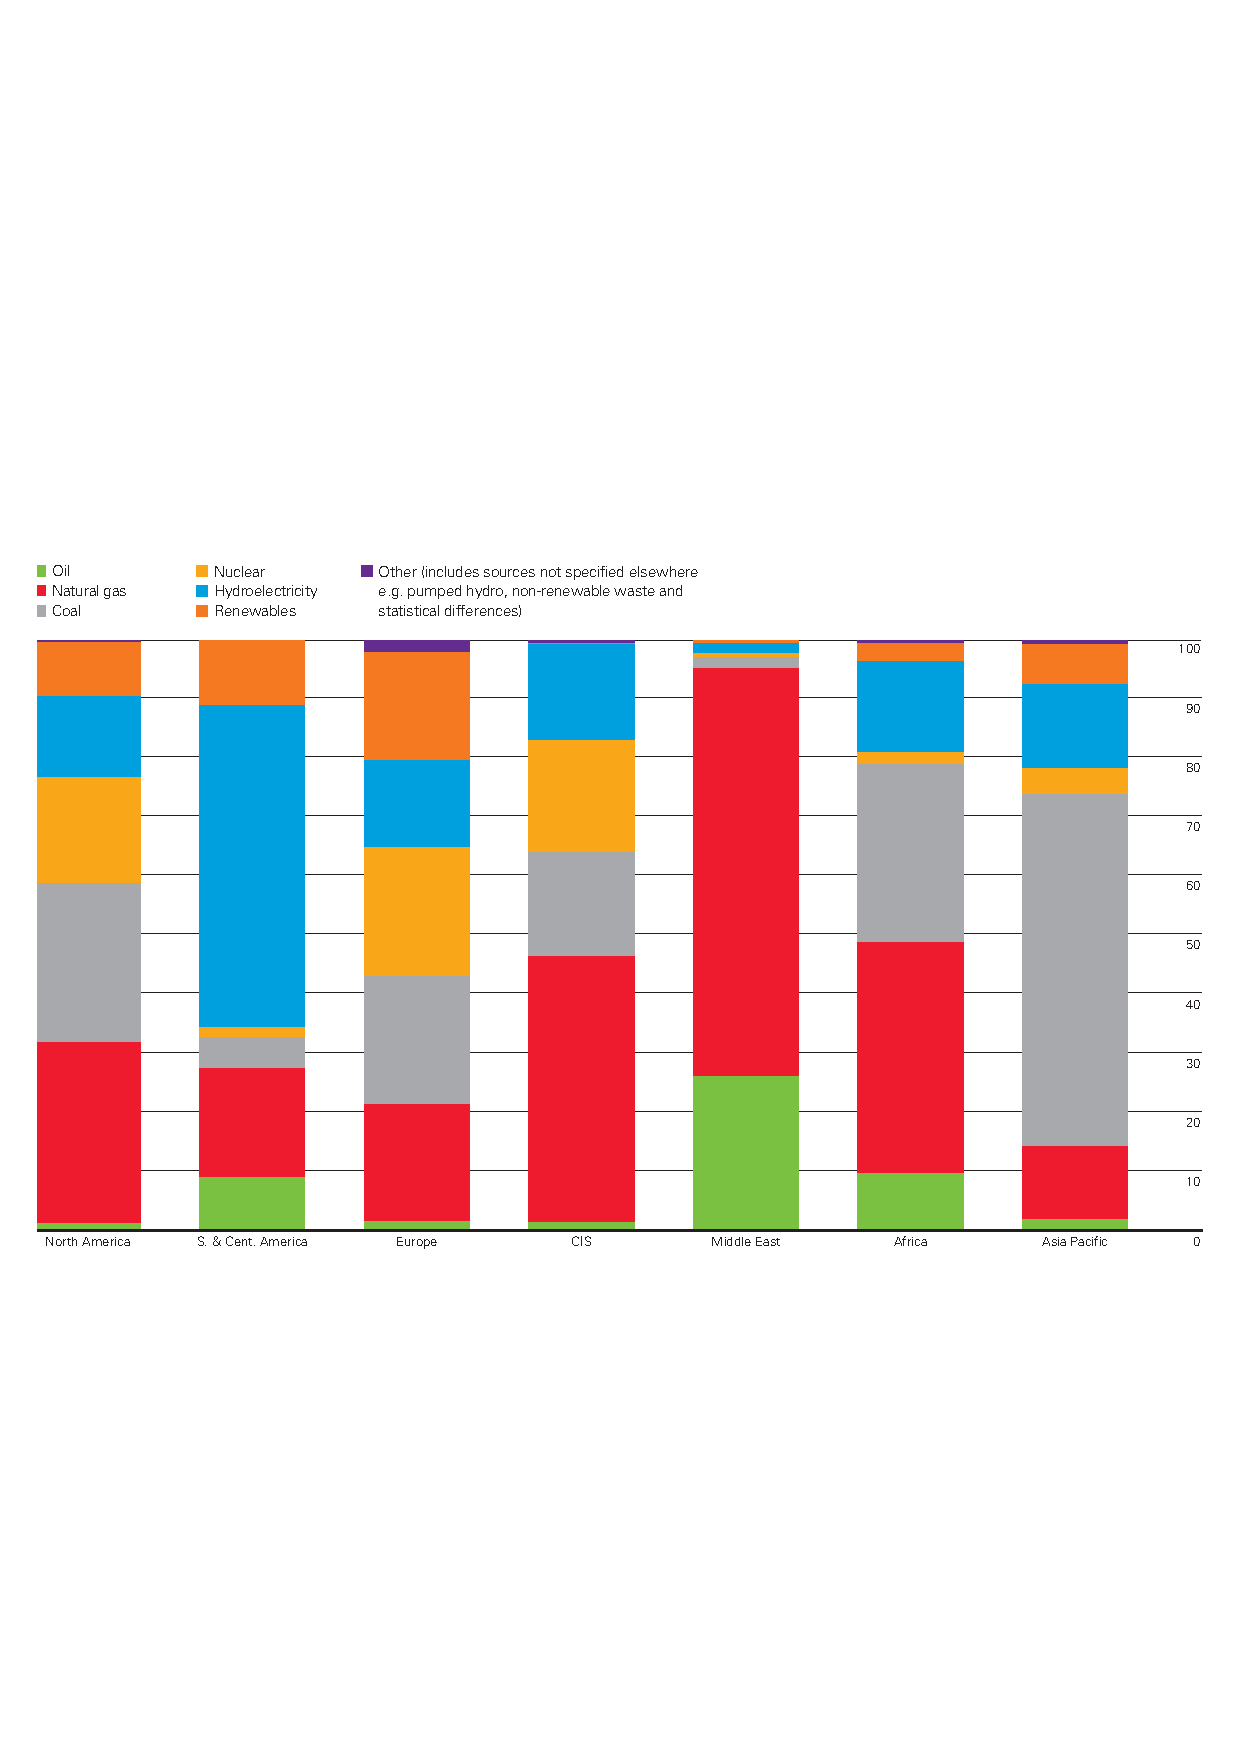
\includegraphics[width=\textwidth]{\figpath/Fig_cap_introduction/Energy_by_continent_2}
	\end{minipage}
		\begin{minipage}{.50\textwidth}
		(b) \\
		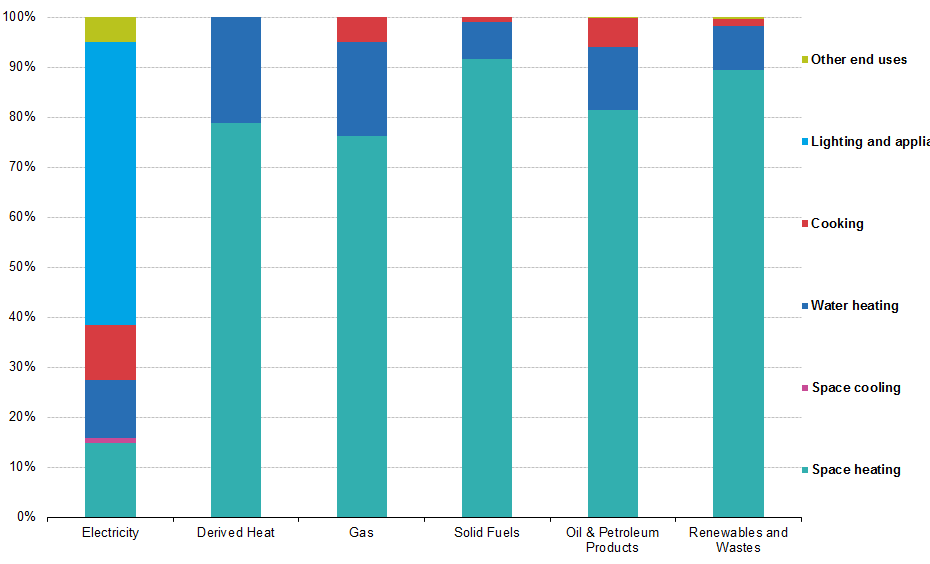
\includegraphics[width=\textwidth]{\figpath/Fig_cap_introduction/Energy-residential-EU}
	\end{minipage}
	\caption{(a) Electricity generation by different energy sources in 2017 by different continent by \cite{dudley2018bp}. (b) Energy use repartition in a residential buildings in Europe by \cite{dudley2018bp}.}
	 \label{fig-Energ-cons}
\end{center}	
\end{figure}

\noindent Research on environment-friendly energy sources, such as biomass, wind or solar have attracted many considerations recently.
Even though solar or wind energy are now operational, their main drawback remains the gap between their availability and the consumers demand.
Solar energy is not available during the nights for example, while wind energy is intermittent over the year.
The energy demand varies with time and the energy suppliers have to meet this demand.

\noindent Current solution to deal with this discrepancies of availability and demands problem is the use of energy storage systems.
The idea is to store the available energy at one time in one form or another and release it latter for a particular need, since energy availability and demand rarely concur.
The energy storage process is a crucial point for renewable and sustainable energy.
The later can be divided into five classes:
magnetic, biological, chemical, mechanical and thermal energy storages.
The main feature of the aforementioned energy storage technologies relies on energy charging and discharging process.
In most cases however, thermal energy is the energy form widely used.
Even the electricity generation is monitored by heat generating high temperature and high pressure.
Storing thermal energy is hence an efficient and fundamental way to store the energy.
It can be realised by rising the substance's temperature (sensible heat energy storage) or by changing the substance's phases (latent heat energy storage).


\begin{table}[!h]
	\begin{center}
		\begin{tabular}{ccccc}
			Agriculture & Buildings & Industry  & Transportation & Other  \\ \hline
			4.5 & 41.8 & 26 & 43.8 & 4.5 \\
		\end{tabular}
	\end{center}
	\caption {The energy consumed by different domain in France in 2017, in million tonne of oil equivalent. French ministry of ecological transition \citep{ministereEcologie2018}.}
	\label{tab-french-min}
\end{table}

\noindent To this end, research on passive heat storage system have attracted many considerations lastly, namely interest on Phase Change Material (PCM) as a latent heat energy storage have arisen.
PCM are used to store heat during the melting of the materials and releases later the stored energy during the solidification process.
At present, the latent heat storage technologies are proven as an effective solution to decrease the use of fossil fuel and in the same time increase the energy usage efficiency.


Aside from energy storage technologies, PCMs are also widely used in building applications, to decrease the temperature fluctuations.
Latest announcement of the french ministry of ecological transition, detailing the repartition of the energy consumption in different domains, indicates more than $35 \%$ of the total energy being consumed by residentials and commercial buildings. Details about energy consumptions in 2017, reported by the french ministry of ecological transition are shown in Tab. \ref{tab-french-min}.
More than $60\%$ of the total energy consumption in residential sector is dedicated to space heating (see Fig. \ref{fig-Energ-cons}b).
Research towards energy-efficient building to reduce heating and cooling demand is of principal interest nowadays.
Taking advantage of the high value of the latent heat of solid-liquid transformations, PCMs are extensively encountered in buildings thermal regulation to reduce overheating.
In summer, PCMs are used to absorb the excessive solar radiation heat and maintain a bracing indoor ambience.
PCM with a temperature of fusion close to the ambient temperature is generally used to ensure melting during the daytime and solidification during the nighttime.
During winter however, PCMs can be used to store heat generated by electrical heating system during the night and then release it in the daytime.

%The use of efficient insulation is the key of energy conservation in residential buildings.

\begin{table}[!h]
	\begin{flushleft}
		\begin{tabularx}{\linewidth}{cXX}
					Temperature range & PCM & Target application area \\ \hline \hline
			0 - 65 $^o C$ &    Paraffins (-3 to 64 $^o C$), water / ice  (0 $^o C$), stearic acide  (41 - 43 $^o C$), {n-octadecane  (27.7 $^o C$)}   &   Storage for domestic heating/cooling. Passive storage in bio-climatic building/architecture. Thermal storage of solar energy. Application in off-peak electricity for cooling and heating. Protection of electrical devices.\\ \hline
			%80 - 120 $^o C$ & Erythritol (117.7 $^o C$), RT100  (99 $^o C$),  $MgCl_2 6H_2 O$& \\ \hline
			80 - 120 $^o C$ &    Erythritol (117.7 $^o C$), RT100  (99 $^o C$), $MgCl_2 \, 6H_2O$  (116.7 $^o C$)   &   Storage for the hot-side of $LiBr/H_2O$ absorption cooling system with generator temperature requirements of less than 120 $^o$C\\ \hline
			$ > 150 $ $^o C$ &    $NaNO_3$ (310 $^o C$), $KNO_3$  (330 $^o C$), $NaOH$  (318 $^o C$),  $KOH$  (380 $^o C$), $ZnCl_2$  (280 $^o C$)  &   Storage for solar power plants based on parabolic trough collectors and direct steam generation.\\ 

		\end{tabularx}
	\end{flushleft}
	\caption {Target application area for some PCM studied in the literature \citep{agyenim2010review}.}
	\label{tab-PCM-app}
\end{table}

PCMs are a very timely subject and is encountered in a wide range of applications ranging from metal casting and passive temperature control devices (e.g. for modern portable electronics), to food freezing and cryosurgery.
In many of these applications, the choice of an appropriate material for a specific end depends of many criteria, such as the operating temperature range, the thermal conductivity, the costs, etc.
They are generally classified into three classes: organic, inorganic and eutectic.
A target application area for some PCM is drawn in Tab. \ref{tab-PCM-app}.
The main operating temperature range can be assorted by three groups. First, $0$ to $65 ^o C$ for thermal storage used in domestic heating/cooling or for thermal storage of solar energy. Paraffins and water are used for such applications.
Second, $80$ to $120 ^o C$ for the cooling of systems with generator temperature of less than $120 ^o C$ purpose.
Finally, greater than $150 ^o C$ for the heat storage in solar power plants based on parabolic trough collectors and direct steam generation.
For more details about these applications see \citep{agyenim2010review}.

Melting and solidification are also fundamental process in geophysical problem such as Earth's mantle formations, lava lakes \citep{davaille1993thermal}, thermal convection in magma chambers \citep{brandeis1989convective} or ice-melt lakes \citep{polashenski2012mechanisms}. Ice-melt ponds that form during summer season in the Arctic are known for example to display natural convection coupled to a phase-change process on the bottom side \citep{polashenski2012mechanisms,esfahani2018basal}. 
In that case, Rayleigh-B�nard like convection cells are observed in the liquid phase.

The solid-liquid phase-change phenomenon is a very complex process. 
It couples the natural convection in the liquid phase induced by the buoyancy force, the non-linear evolution of the phase-change interface and the heat transfer process, which could be different from one configuration to another.
The coupling of all these physical phenomenons induces strong non-linear process in the solid-liquid problems, difficult to analyse except for simple and ideal test cases.
Fig. \ref{fig:expe-PCM_Gong} showing the experimental investigation of the melting of n-octadecane inside a transparent brick by \cite{gong2015numerical} displays very well the complexity of the problem.
The investigated material is heated from the right and melts from the right to the left.
Figs. \ref{fig:expe-PCM_Gong}a and \ref{fig:expe-PCM_Gong}b indicate the evolution of the liquid fraction and the vector field in the fluid obtained by particle image velocimetry (PIV) method.
Capturing accurately the non-linear evolution of the solid-liquid interface, due to the strong convection in the melting PCM, is clearly a challenging numerical task.
Furthermore, the existence of boundary layers near the walls and the interface suggests that the mesh resolution should allow to capture these structures.

\begin{figure}[!h]
	\begin{center}
		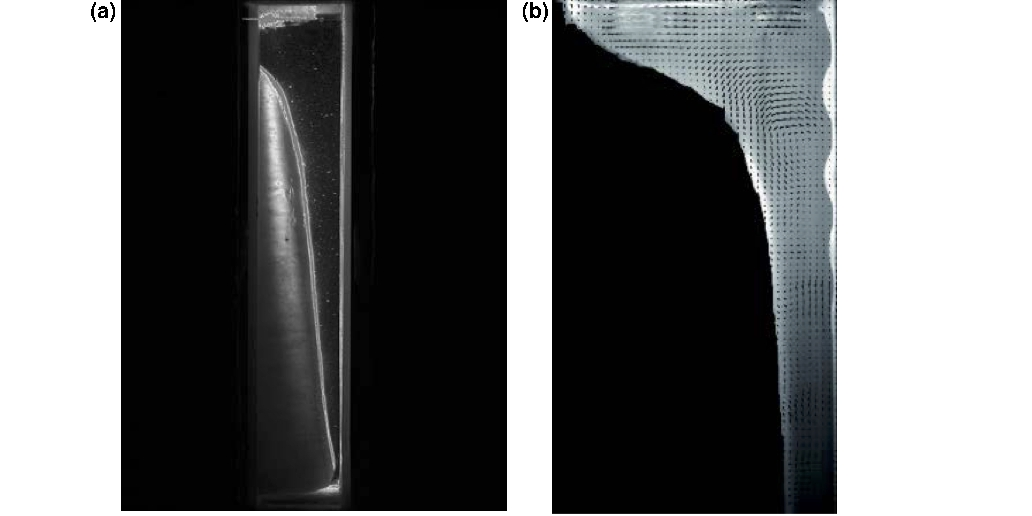
\includegraphics[width=\textwidth]{\figpath/Fig_cap_melting/EXPE_GONG_melting}
	\end{center}
	\caption{Experimental observation of the melting of n-octadecane within a transparent brick of plexiglas heated vertically from the left by \cite{gong2015numerical}, obtained by particle image velocimetry (PIV) method.}
	\label{fig:expe-PCM_Gong}
\end{figure}

Over the past $30$ years, solid-liquid phase-change has been widely studied. % using either numerical, analytical, or experimental methods.
Rectangular and cylindrical geometries were the most investigated configuration.
\cite{Okada1984,gau1983flow,gong2015numerical} have investigated experimentally the melting of n-octadecane and gallium PCMs inside rectangular containers.
\cite{ho1984inward,liu2014experimental,omojaro2017study} have studied experimentally the melting of different paraffin within cylindrical enclosures.
These experimental investigations have been extensively used for numerical validations (see \cite{bertrand1999melting,gobin2000melting,wang2010numerical,dan-2014-JCP,rakotondrandisa2019numerical}) and have permitted a better comprehension of the physical phenomenon that occurs during melting and solidification, mainly the heat transfer process.
%The experimental results are very often formulated in the form of mathematical correlations.
Experimental work of \cite{Okada1984} have permitted for example to express correlations of the variation of dimensionless thermal energy stored as latent heat, and the average Nusselt number on the vertical wall with the dimensionless time.
Later, \cite{ho1984inward} have analyzed the solid-liquid interface position for different configuration and \cite{jany1988scaling} have formulated $N\!u$-$\Ray$ correlation through a scaling analysis.
\cite{bejan1989analysis} gathered the previous observations and described analytically the solid-liquid melting process in the frame of vertical heating.

Gallium and n-octadecane are the most investigated materials. Experimentals \citep{gau1983flow,Okada1984,campbell1994visualization,gong2015numerical}, numericals \citep{rady1996natural,bertrand1999melting,hannoun2003resolving,Wang2010,dan-2014-JCP,rakotondrandisa2019numerical}, and theoreticals \citep{Okada1984,jany1988scaling,bejan1989analysis,kowalewski2004phase} works were  performed. 
Besides their physical properties are equal in both liquid and solid phases (differences less than $3 \%$), gallium and n-octadecane melt near room temperature, making them the preferred materials for experimentally investigating melting and solidification of low and high Prandtl-number PCMs respectively.
%These problems in a rectangular cavity have been also extensively used in the literature for the assessment of phase-change numerical methods

The previously mentioned works were mostly focused on studying separately melting or solidification problems
and only recently for alternate melting and solidification complete cycles \citep{wang2010numerical,rakotondrandisa2019numerical}. 
Prior to these studies on complete cycles, periodic melting and solidification problems were the most studied in the literature. 
\cite{ho1993periodic} and \cite{voller1996cyclic} studied numerically, periodic melting in square enclosures. 
Recently, \cite{hosseini2014experimental} carried out melting and solidification of a cylindrical PCM during charging and discharging process and \cite{chabot2017solid} studied analytically the effect of an alternate heating and cooling in a cylindrical PCM, with periodical boundary conditions.
We have also contributed recently on the comprehension of the governing mechanism during the melting and the solidification process in the paper \cite{rakotondrandisa2019numerical}.
We analysed in detail the difference between solidification occuring after a partial melting and a complete melting by providing temporal evolution of solid-liquid interface, liquid fraction, Nusselt number and accumulated heat input. 

While publication about melting and solidification of PCM heated from the side is very abundant, research on melting of PCM heated from below is quite rare.
\cite{diaz1984visualization,hale1980solid} have studied experimentally the solid-liquid interface morphology of PCM during basal heating.
\cite{gong1998flow} studied numerically the flow and heat transfer during the melting of pure n-octadecane in a rectangular cavity heated from below.
Recent numerical simulations have investigated different boundary conditions such as
periodic configurations along the horizontal axis \citep{esfahani2018basal,madruga2018dynamic,favier2019rayleigh} or wavy surface in a rectangular cavity heated from below \citep{kousksou2014melting}.
With regard to theoretical works, \cite{vasil2011dynamic,favier2019rayleigh} have studied the hydrodynamic instabilities at the onset of convection and compared their observation with the classical Rayleigh-B�nard instability mechanism \citep{chandrasekhar2013hydrodynamic}.
\cite{favier2019rayleigh} have focused their attention to the effect of the non-planar topography of the interface to the convection flow.
 On the other hand, \cite{gong1998flow,esfahani2018basal,madruga2018dynamic} mostly focused on global quantities such as the heat flux and the statistical properties of the interface.


\section{Purpose of the thesis}
The purpose of the present work is to investigate numerically solid-liquid phase-change systems.
The investigation tool used in this thesis is the open-source software FreeFem++ \citep{freefem,hecht-2012-JNM}.
A high accuracy numerical model using a Newton method with an adaptive finite element is used to simulate phase-change problems involving natural convection.

\noindent A first investigation on the numerical simulation of convective phase-change problems using adaptive finite element method have been carried out by \cite{dan-2014-JCP}.
The method used consists of solving the Navier-Stokes-Boussinesq equations by the mean of single domain approach using first order scheme.
The technique of variable viscosity approach was applied to annihilate the velocity in the solid phase.
The study was focused on two-dimensional square cavity configuration.

A first objective of this thesis is to improve the existing code, developed by the numerical methods and applications group of the LMRS Laboratory \footnote{http://lmrs-num.math.cnrs.fr}, and to organize the program as a toolbox for the software FreeFem++.
To this end, the objectives are listed as follows: 
\begin{enumerate}[label=(\roman*)]
\item increase the accuracy by using  a second order scheme for the time discretization and P$_2$ finite element for the temperature, 
\item implement a Carman-Kozeny model, in addition to the viscosity-based approach, to annihilate the velocity in the solid region, 
\item investigate challenging cases by simulating complex geometries (highly distorted mesh, cylindrical PCM with inner heated tubes) and computationally demanding cases (high Rayleigh numbers), 
\item simulate the complete melting-solidification cycle of a PCM. 
\end{enumerate}
A second objective is to extend the program to three-dimensional configurations.
The two dimensional assumption is indeed no more valid for high Rayleigh problems, especially for basal melting cases.
Moreover, three dimensional adaptive finite element method for convective melting problem is less investigated in the literature.

A third objective is to provide a thorough analysis of both melting and solidification process using the developed tools.

\newpage
\subsection{Existing method for modeling phase-change materials}
%Solid-liquid phase-change problems are encountered in numerous practical applications, ranging from metal casting and thermal energy storage (phase-change materials) to food freezing and cryosurgery. Melting and solidification are also fundamental processes in geophysical problems, such as Earth's mantle formation, lava lakes or magma chambers. 

Temperature gradients induce buoyancy forces in the liquid (melted) phase and generate a significant convective flow.
The appropriate mathematical description of the liquid phase is thus the usual model for the natural convection flow: the incompressible Navier-Stokes system of equations  with Boussinesq approximation for thermal (buoyancy) effects (\eg \cite{viskanta1985natural}). 
In this model, the energy conservation equation is written as a convection-diffusion equation for the temperature. 
In the solid phase, conduction is the main phenomenon and the appropriate model is the classical heat equation. 
The main modelling difficulty is to link these two models by taking into account the separation of the two phases by a sharp interface, across which thermodynamic properties are discontinuous. 

We offer in this section a description of the two main approaches suggested in the literature to deal with solid-liquid phase change problem.  
For a comprehensive review of models for phase-change problems with convection, see \cite{kowalewski2004phase}.  Note that a different category of models was recently suggested in the literature, based on the Lattice Boltzmann Method \citep{luo2015lattice,gong2015numerical} or meshless methods \cite{atluri2002meshless}.  Such methods based on non-deterministic models are not discussed in this introduction.

A first modelling  approach, usually referred to as the multi-domain (or deforming-grid) method, is based on the classical Stefan two-phase model. Solid and liquid domains are separated and the corresponding conservation equations are solved in each domain. Boundary conditions at the interface between domains are obtained by imposing the Stefan condition (balance  of heat fluxes at the interface). The position of the solid-liquid interface  is tracked and moved explicitly using  either {\em front tracking} or  {\em front fixing} methods. The  former method uses deforming grids to reconstruct the interface, while the latter is based on a time-depending coordinate transform, mapping the physical domain into a fixed computational domain. For a detailed description of these methods, see \eg \cite{sparrow1977analysis,unverdi-JCP-1992,gupta2000moving,Tenchev2005}. The main drawback of deforming-grid methods is their algorithmic complexity, which makes difficult to accurately capture solid-liquid interfaces of complicated shape or structure (\eg with mushy regions between solid and liquid phases). Configurations with multiple interacting interfaces (see the solidification of a phase-change material presented in this work) are also difficult to simulate with these methods (see also \cite{kowalewski2004phase-stella}). 

The second modelling approach avoids to impose explicitly the Stefan condition at the solid-liquid interface and therefore uses a single-domain (or fixed-grid) model. The same system of equations is solved in both liquid and solid phases. The energy balance at the interface is implicitly taken into account by the model. Consequently, the position of the interface is obtained a posteriori by post-processing the computed temperature field. Phase-field methods \citep{fabbri-JCP-1997} and enthalpy methods \citep{Voller-1987,Cao1989} are the most commonly used single-domain models. In phase-field methods, a supplementary partial differential equation for the evolution of the order parameter (a continuous variable taking the value 0 in the solid and 1 in the liquid) has to be solved, coupled with the conservation laws \citep{shyy-1996}. This new equation is model dependent and its numerical solution could lead to diffuse solid-liquid interfaces.  For recent contributions in this area, see \cite{boettinger2002phase,singer2008phase,favier2019rayleigh}. We focus below on enthalpy methods, which are the most widely used single-domain models due to their algorithmic simplicity. 

\noindent The main idea behind enthalpy models is to formulate the energy conservation law in terms of enthalpy and temperature and include latent heat effects in the definition of the enthalpy. The obtained equation applies to both liquid and solid phases and implicitly takes into account the separation of the phases. Another advantage of enthalpy methods, when compared to previously described models, is to  remove the limitation of the phase-change occurring at a fixed temperature. The presence of mushy regions can be easily modelled  with these methods. Two types of formulations of enthalpy methods exist in the literature, depending on the main variable used to solve the energy equation: enthalpy or temperature-based methods. \\
In enthalpy-based formulations  the main variable is the enthalpy \citep{eyres1946calculation,rose1960method,bhattacharya2014enthalpy}.  Temperature is computed  from the temperature-enthalpy coupling model. An iterative loop is necessary to solve the energy equation, formulated with both enthalpy and temperature variables. For a review of different iterative techniques to solve the energy equation, see \cite{Voller-1996-chapter}.  A second variety of enthalpy-based formulations consists in rewriting the energy equation with enthalpy terms only \citep{rady1996natural,hannoun2003resolving}. \\
In temperature-based formulations, the energy equation is formulated in terms of temperature only. The latent heat is  treated either by deriving an apparent heat capacity coefficient to define the total enthalpy \citep{Morgan-1978,chiesa1974natural,gau1984melting}  or by introducing a source term in the energy equation \citep{Voller-1996-chapter,swaminathan1997towards}. Advantages and drawbacks of each approach are discussed in detail in \cite{konig2017comprehensive}.

Single-domain methods are very appealing for numerical implementations. The same system of equations is solved in the entire computational domain, making possible algorithmic or computer-architecture optimisations. If enthalpy models offer an elegant solution to deal with the same energy conservation equation in both phases, a last modelling problem has to be solved. It concerns the  extension of the  Navier-Stokes-Boussinesq equations from the  liquid to the solid phase. 
Different techniques to bring the velocity to zero in the solid region were suggested. 

\noindent The most straightforward is the switch-off technique, which decouples solid and liquid computational points and overwrites the value of the velocity by setting it to zero in the solid region. Different implementations of this technique with finite-volume methods are presented in \cite{Ma2006,Wang2010}. 

\noindent In variable viscosity techniques \citep{gartling-1980,voller1987pcm,Cao1990}, the fluid viscosity depends on the temperature and is artificially increased to huge values in the solid regions through a regularisation or mushy zone. To avoid blow-up or numerical inconsistencies, the large gradients of viscosity must be correctly resolved in the mushy region.  
This is naturally achieved in finite-element methods with dynamical mesh adaptivity   \citep{dan-2014-JCP}, while in finite-volume methods with fixed grids, the time step has to be adapted to the space resolution \citep{Ma2006}. Versions of the variable viscosity approach suggested in  \cite{dan-2014-JCP} were further studied by \cite{aldbaissy2018full,WOODFIELD-2019} and implemented in a different finite-element framework (FEniCS) by \cite{zimmerman-2018}.

\noindent A third technique used to ensure a zero velocity field in the solid phase is the so-called enthalpy-porosity model \citep{Brent-1988}.  A penalisation source term is introduced in the momentum equation to allow the switch from the full Navier-Stokes equations in the liquid phase to a Darcy equation for porous media. The mushy region is thus regarded as a very dense porous medium that sharply brings the velocity to zero in the solid region. The expression of the penalisation source term generally follows the Carman-Kozeny model for the permeability of  a porous medium \citep{hannoun2003resolving,hannoun2005,Belhamadia2012}, but other mathematically equivalent expressions were suggested \citep{Angot-1999,favier2019rayleigh}. Different formulations and implementations of the enthalpy-porosity model are presented in \cite{Kowalewski-1999,Giangi-2000,kowalewski2004phase-stella}.

Concerning the space discretization of these models, finite difference (FD) or finite volume (FV) methods are generally used in the literature. 
When single-mesh models are used, the general strategy to capture the solid-liquid interface is to dramatically increase the mesh resolution in the whole domain. 
This results in a considerable increase of the computational time, even for two dimensional cases. 
 \citep{hannoun2003resolving} have reported that the simulation of the melting of tin within $200 \times 200$ fixed grid  required $2,400$ CPU hours, $111$ runs (restarts), and $3$ months of calculations.
Dynamical mesh adaptivity becomes in this context a valuable tool  to concentrate the grid refinement effort only in regions displaying high gradients of the computed variables (melting-solidification fronts, thermal or viscous boundary layers, recirculation zones). 

\noindent Finite  element (FE) methods offer this possibility to dynamically refine the mesh only in specific regions of the domain. %where sharp phenomena takes place (\eg solid-liquid interface, recirculation zones). 
Different FE approaches were suggested, from enthalpy-type methods (\eg \cite{elliott1987error}) to front-tracking methods (\eg \cite{CHLi}). 
Recently, adaptive FE methods were proposed for classical two-phase Stefan problem \citep{Belhamadia2004_S} using an anisotropic mesh adaptation algorithm based on solution-dependent metrics.
The authors extended  their algorithm for the three-dimensional simulation of the same problem  \citep{Belhamadia2004_3D} and showed that the use of locally adapted meshes with strong anisotropy proved to be very effective in reducing the number of computational nodes for such phase-change systems without convection.

\noindent To simulate melting or solidification problems with convection,  \cite{dan-2014-JCP}  recently suggested a dynamical mesh adaptation algorithm based on metrics control and implemented with the \ff software \citep{freefem,hecht-2012-JNM}. 
%and phase-change systems with convection  \citep{Belhamadia2012,dan-2014-JCP}. 
%For the classical two-phase Stefan problem, \cite{Belhamadia2004_S} suggested  an anisotropic mesh adaptation algorithm based on solution-dependent metrics. 
The advantage of this adaptive finite-element method, which will be also used in the present study, is to make possible, with reasonable computational cost, the re-meshing of the computational domain at each time step. 
A very refined discretization of the  regularization zone between solid and liquid phases is thus obtained, while regions with low gradients are de-refined in order to balance the overall computational effort. 

\subsection{Present numerical approach for modeling phase-change materials}
The present work is based on a single-domain enthalpy-porosity model for solid-liquid phase change problems with convection. 
For the energy conservation equation, a temperature-based formulation takes into account the latent heat by introducing  a discontinuous source term. 
For the mass and momentum conservation equations, we solve in the entire domain the incompressible Navier-Stokes equations with Boussinesq approximation for buoyancy effects. 
To bring the velocity to zero in the solid phase, we introduce in the momentum equation a penalty term following the Carman-Kozeny model.  
The coupled system of momentum and energy equations is integrated in time using a second-order Gear scheme. 
All the terms are treated implicitly and the resulting discretized equations are solved using a Newton method \citep{dan-2014-JCP}. 

\noindent The advantage of this formulation is to  permit a straightforward implementation of different types of non-linearities.
For the space discretization we use Taylor-Hood triangular finite elements, \ie P$_2$ for the velocity and P$_1$ for the pressure. 
Temperature is discretized using P$_2$ or P$_1$ finite elements. 
Discontinuous variables (latent heat, thermal diffusivity, etc) at the solid-liquid interface are regularized through an intermediate artificial mushy region.

\noindent Single domain methods require a refined mesh near the interface, where large enthalpy gradients have to be correctly resolved. 
An optimized dynamical mesh adaptivity algorithm allows us to adapt the mesh every time step and thus accurately capture the evolution of the interface.  
Mesh adaptivity, feature of the current method, offers the possibility to deal with complicated phase-change cases, involving multiple solid-liquid interfaces.

\noindent There are three main novelties in the present numerical approach, when compared to  \cite{dan-2014-JCP}: 
\begin{enumerate}[label=(\roman*)]
\item we use the Carman-Kozeny model to bring the velocity to zero inside the solid phase, instead of a  viscosity penalty method (imposing a large value of the viscosity in the solid), 
\item we increase  the time accuracy of the algorithm by replacing the first-order Euler scheme with the second-order Gear (BDF2) scheme (see also \cite{Belhamadia2012}), 
\item we improve the metric calculation procedure for mesh adaptivity.
\end{enumerate}

The programs were built and organized as a toolbox for \ff \citep{hecht-2012-JNM,freefem}, which is a free software (under LGPL license). \ff\footnote{\ff for different OS can be downloaded from \texttt{http://www3.freefem.org/}.} offers a large variety of triangular finite elements  (linear and quadratic Lagrangian elements, discontinuous P$_1$, Raviart-Thomas elements, etc.)  to solve partial differential equations. It is an integrated product with its own high level programming language and a syntax close to mathematical formulations, making the implementation of numerical algorithms very easy. Among the features making \ff an easy-to-use and highly adaptive  software we recall the advanced automatic mesh generator, mesh adaptation, problem description by its variational formulation, automatic interpolation of data, colour display on line, postscript printouts, etc. The \ff programming framework offers the advantage to hide all technical issues related to the implementation of the finite element method. It becomes then easy to  use the present toolbox to code new numerical algorithms for similar problems with phase-change.

%In this thesis, we use an enthalpy method with a temperature-based formulation using heat source term approach to simulate phase-change systems with convection.
%The natural convection flow in the liquid phase is simulated by solving the full incompressible Navier-Stokes equations with Boussinesq approximation.
%A Carman-Kozeny type penalty model is applied to ensure a zero velocity value in the solid region.
%The main feature of our numerical approach is the use of an adaptive finite element method to accurately track the solid-liquid interface.
%Single domain method requires actually a fine mesh near the phase change front in order to capture the large enthalpy gradient. 
%The smaller the phase change interval the narrower the mushy region and the more refined the mesh should be.
%Yet applying a fine mesh in the whole domain would increase considerably the computational time.
%Hence, we introduce a FE method with time-dependent mesh adaptivity by metric control that is  effective for a large range of phase-change systems with convection, from melting to solidification. The proposed mesh refinement strategy has the capacity to take into account different metrics and thus the ability to refine the mesh in different regions of interest in the computational domain. In particular, we show that the method is able to simultaneously track several interfaces in the domain.\\ 
%The nonlinear system of equations are solved by means of a Newton algorithm.
%A fully-implicit Newton method for the phase-change system based on a finite-element formulation of the Navier-Stokes equations has been derived by \citep{dan-2014-JCP}.
%The advantage of this formulation is to  permit a straightforward implementation of different types of non-linearities in the system of equations.
%
% The code was built as a toolbox for FreeFem++ \citep{hecht-2012-JNM,freefem}, which is a free software (under LGPL license) using a large variety of triangular finite elements  (linear and quadratic Lagrangian elements, discontinuous P$_1$, Raviart-Thomas elements, etc.)  to solve partial differential equations. FreeFem++ is an integrated product with its own high level programming language and a syntax close to mathematical formulations, making the implementation of numerical algorithms very easy. Among the features making FreeFem++ an easy-to-use and highly adaptive  software we recall the advanced automatic mesh generator, mesh adaptation, problem description by its variational formulation, automatic interpolation of data, colour display on line, postscript printouts, etc. FreeFem++ community is continuously growing, with  thousands of users all over the world.

\section{Thesis plan}
Chapter \ref{chap-NSB} sets the mathematical and physical basis of the numerical system used to simulate phase-change problems involving natural convection flow.
We present in detail the incompressible Navier-Stokes-Boussinesq equation and the single-domain approach to solve the same system of equations throughout the whole domain.
The enthalpy method, modeling the phase-change phenomenon is presented first.
The Navier-Stokes equation with Boussinesq approximation to simulate the natural convection in the liquid flow is then developed.
Finally, the final non-dimensional system of equations is described in detail with a discussion about the Carman-Kozeny model used as a penalty term in the momentum equation.

Chapter \ref{chap-FEM} is devoted to the numerical algorithm for solving the numerical system presented previously.
The finite element algorithm we have developed in this work is first presented in detail: time integration scheme, finite element discretization and the Newton method.
The characteristics Galerkin method, an alternative for the treatment of non-linear term in the momentum equation, is also presented.
Then, we describe the mesh adaptivity by metric control, which is a standard function offered by FreeFem++.
Some theoretical tests to assess for the accuracy of our numerical method is also presented.
The space and the time convergence orders are demonstrated using the Burggraf flow and a manufactured solution designed for the incompressible Navier-Stokes equation.
The structure of the new finite-element toolbox for the simulation of PCMs is also described.
The program architecture and the parameter details are presented.
Finally, the domain decomposition method used for large scale simulation is described.

A first validation of our numerical method is addressed in Chapter \ref{chap-NATCONV}.
The capability of the code to deal with linear and non-linear forms of the buoyancy force in the Boussinesq approximation is first tested.
%Differentially heated cavity (horizontal $\nabla T$) configuration is used to compare our results with benchmarks solution existing in the literature.
The test cases are presented by increasing progressively the difficulty.
We simulate first the natural convection of air in square enclosures differentially heated from the vertical walls.
Then heated obstacle is added in the center of the domain.
Finally, we add non-linearity by simulating the natural convection of water.
%Three-dimensional simulations of the natural convection of air is also presented.
%For both two and three-dimensional configurations, qualitative and quantitative validations are provided.

Once the capability of our algorithm to deal with natural convection issues was demonstrated, much more attention to phase-change problem is paid.
Numerical simulation of melting and solidification of PCM is considered in Chapter \ref{chap-MELTING}.
The melting of octadecane and gallium inside rectangular enclosures are investigated first since they were extensively used for numerical method validations, because of their physical properties relatively equal in both solid and liquid phases.
Finally, several PCM container geometries are simulated to prove the robustness of our numerical method, mainly cylindrical and irregular domain are computed.
%Finally, numerical simulation of three-dimensional configuration is presented.

Numerical and scale analysis are investigated in Chapter \ref{chap-MELTING-ANALYSIS}.
We compare the behavior of the PCM when lateral and basal heating are of interest.
The melting of octadecane heated from the side is carried out first.
Then numerical results for the melting from below is performed.
For  both cases, we provide detailed description of the melting process with scaling analysis to better understanding the heat transfer mechanism.
%Accurate comparison is carried out for the differentially heated cavity case, by considering different size of the cavity and different temperature difference between the hot temperature and the temperature of fusion, which are the main parameters monitoring the natural convection in the melting PCM.
Analysis of the time evolution of some physical parameters, such as the Nusselt number, the liquid fraction, the accumulated heat input and the time evolution of the melting are discussed. %provided in detail through a scaling analysis.

Chapter \ref{chap-SOLIDIFICATION} displays the numerical simulation of a full cycle melting/solidification of a PCM. 
Two solidification fronts have to be tracked and make the case very challenging.
A differentially heated cavity case and a circular PCM with inner heated tubes are studied.
A comparison on the influence of the Rayleigh number during the melting and the solidification process is emphasized, since both cycles are not driven by the same mechanism.

Chapter \ref{chap-3D-SIMULATION} is devoted for three-dimensional configurations simulated using parallel algorithm.
3D simulations of PCM are indeed less investigated in the literature.

Finally, Chapter \ref{chap-conclusion} draws the conclusion of this study and some perspectives for future developments.



%%%%%%%%%%%%%%%%%%don't forget if needed %%%%%%%%%%%%%%%%%%%%%
%\section[toc version]{title version%
%              \sectionmark{head version}}
%\sectionmark{head version}
%%%%%%%%%%%%%%%%%%%%%%%%%%%%%%%%%%%%%%%%%%%%%%%%%%%%%%%%%%%%%%
\def\titcourt{Numerical resolution of the Navier-Stokes-Boussinesq model}
\def\titlong{Numerical resolution of the Navier-Stokes-Boussinesq model}
%%%%%%%%%%%%%%%%%%%%%%%%%%%%%%%%%%%%%%%%%%%%%%%%%%%%%%%%%%%%%%%%
\chapter[\titlong]{\titlong%
              \chaptermark{\titcourt}}
\chaptermark{\titcourt}
\label{chap-NSB}
%%%%%%%%%%%%%%%%%%%%%%%%%%%%%%%%%%%%%%%%%%%%%%%%%%%%%%%%%%%%%%%%
%%%%%%%%%%%%%%%%%%%%%%%%%%%%%%%%%%%%%%%%%%%%%%%%%%%%%%%%%%%%%%%%

\section{Governing equations} \label{sec-gov-eq}
%%%%%%%%%%%%%%%%%%%%%%%%%%%%

We consider a solid-liquid system placed in a two-dimensional square cavity of height $H$. In the following, subscripts $s$ and $l$ will refer to the solid and liquid phases, respectively. 

For the numerical implementation, it is convenient to adopt a single-domain approach to describe both phases using the same system of equations. 
The model is based on the Navier-Stokes equations with Boussinesq approximation, which is the natural description of the fluid flow with natural convection. 
A penalty term is added to the momentum equations to bring the velocity to zero inside the solid region. 
For the energy conservation equation, an enthalpy method is used to model the phase change process. The single-domain model is described in detail in the following sections.

\subsection{Enthalpy method}

The phase change process is modelled using an enthalpy method \citep{voller1987pcm,Cao1989,Cao1990} with temperature-based formulation. We start from the energy equation:
\begin{equation}
\label{eq-energie}
   \frac{\partial (\rho h)}{\partial t_{\varphi}} + \nabla \cdot(\rho h \vec{\tilde{u}}) - \nabla \cdot (k \nabla T) = 0,
\end{equation}
where $t_{\varphi}$ is the physical time, $h$ the enthalpy, $\rho$ the density, $\vec{\tilde{u}}$  the velocity vector, $T$ the temperature and $k$ the thermal conductivity. 
To make Equation (\ref{eq-energie})  valid for the entire domain containing both liquid and solid phases, the total enthalpy $h$ is regarded as the sum of the sensible heat and the latent heat:
\begin{equation}
\label{eq-enth-model}
  {{h}} = c ( T + s(T) ),
\end{equation} 
with $c$ the local specific heat. The function $s(T)$ is introduced to model the jump of the enthalpy due to the phase change and is theoretically a Heaviside step function depending on the temperature: it takes the zero value in the solid region and a large value in the liquid, equal to $h_{sl}/c$, with $h_{sl}$ the latent heat of fusion. 
Linear  \citep{voller1987pcm,Wang2010} or smoother functions \citep{dan-2014-JCP} can be used to regularize $s(T)$ and also the jump of material properties (from solid to liquid). 
In this paper we use a regularization of all step-type functions by a continuous and differentiable hyperbolic-tangent function suggested by \cite{dan-2014-JCP} (see below). 
\Blue{%Moreover, we assume that the undercooling problem is here negligible since only pure and homogeneous materials are considered.
We assume moreover that the undercooling phenomenon is negligible (see also \cite{wang2010numerical,kowalewski2004phase}).}

Equation (\ref{eq-energie}) can be further simplified by considering the following assumptions: (i) the density difference between solid and liquid phases is negligible, \ie $\rho_l=\rho_s=\rho$ is constant; (ii) the regularization zone is narrow and the velocity inside this zone is very low. 
Consequently, the final expression of the energy equation is obtained by combining (\ref{eq-enth-model})  and (\ref{eq-energie}) and  neglecting the convection term $\nabla \cdot ( c s \vec{\tilde{u}})$\footnote{In the liquid phase, $\nabla \cdot ( c s \vec{\tilde{u}})  = h_{sl} \nabla \cdot  \vec{\tilde{u}}=0$; in the solid phase, $s=0$; in the regularization region, it is assumed that $\vec{\tilde{u}}=0.$}:
\begin{equation}\label{eq-energie-enth-model}
\frac{\partial \left(c T\right)}{\partial t_{\varphi}} + \nabla \cdot\left( c T \vec{\tilde{u}}\right) -
\nabla \cdot\left( \frac{k}{\rho} \nabla T \right) +  \frac{\partial \left(c s\right)}{\partial t_{\varphi}}  = 0.
\end{equation}
Furthermore, the essential feature of the current approach is that the phase change front is not tracked explicitly but is instead recovered a posteriori from the computed temperature field.


\subsection{Navier-Stokes equations with Boussinesq approximation}
 

The natural convection in the liquid part of the system is modelled using the incompressible Navier-Stokes equations, with  Boussinesq approximation for buoyancy effects. To make this model valid for both liquid and solid phases, the momentum equation is modified as follows:
\begin{equation}\label{eq-momentum-conserv}
  \frac{\partial \vec{\tilde{u}}}{\partial t_{\varphi}} +   {(\vec{\tilde{u}}\cdot\nabla) \vec{\tilde{u}}} + \frac{1}{\rho}\nabla p - \frac{\mu_{l}}{\rho}  {\nabla^2 \vec{\tilde{u}}} 
- f_B(T) \vec{e}_y= A(T) \vec{\tilde{u}},
\end{equation}
where $p$ denotes the pressure, $\mu_{l}$ the dynamic viscosity of the liquid (assumed to be constant)  and
$f_B(T)$ the Boussinesq force. 
The penalty term $A(T) \vec{\tilde{u}}$ is artificially introduced in (\ref{eq-momentum-conserv}) to extend this equation in the solid phase, where the velocity, pressure, viscosity and Boussinesq force are meaningless.  Consequently, $A(T)$  is modelled to vanish in the liquid, where the Navier-Stokes-Boussinesq momentum equation is recovered. A large value of $A(T)$ is imposed in the solid, reducing the momentum equation (\ref{eq-momentum-conserv})  to $A(T) \vec{\tilde{u}}=0$, equivalent to $\vec{\tilde{u}}=0$. Exact expressions for $f_B$ and $A$ will be given in the next section.

Finally, the conservation of mass in the liquid phase is expressed by the continuity equation:
\begin{equation}\label{eq-mass-conserv}
\nabla \cdot \vec{\tilde{u}} = 0.
\end{equation} 


\subsection{Final system of equations for the single-domain approach}\label{sec-eq-scaling}

It is convenient to numerically solve a dimensionless form of the previous equations.
Using the cavity height $H$ as length scale and a reference state $(\rho, V_{ref}, T_{f})$, we can define the following scaling for the space, velocity, temperature and time variables:
\begin{equation}\label{eq-adim}
\vec{x} = \frac{\vec{\tilde{x}}}{H} \, , \,  \vec{u} = \frac{\vec{\tilde{u}}}{V_{ref}} \, , \,  \theta = \frac{T-T_{f}}{\delta T} \, , \,  t = \frac{V_{ref}}{H} \, t_{\varphi},
\end{equation}
Temperatures $T_h$ (hot) and $T_c$ (cold) will be used to set isothermal walls of the cavity. The difference $\delta T=T_{h}-T_{f}$, with $T_f$ the temperature of fusion, is considered as the representative temperature scale  for the natural convection onset in the liquid region. \Blue{As far as the solidification process is concerned, a distinct discussion will be provided in section \ref{sec-solidification}. } % during the melting,  and $\delta T = T_f - T_c$ during the solidification. }
Thus $\delta T$ is used to define the Rayleigh number of the flow:
\begin{equation}
\label{eq-Rayleigh}
\Ray = \frac{g \beta H^3 \delta T}{\nu_l \alpha_l},
\end{equation}
where $\alpha = k/(\rho c)$ is the thermal diffusivity and  $\beta$ the thermal expansion coefficient. Note that the reference temperature in this scaling is   $T_f$, resulting in  $\theta_f = 0$. This simplifies the identification of the regularization zone, defined for  $  -\varepsilon \, \leq \theta \leq \,\varepsilon $.

Finally, the dimensionless system of equations to be solved in both liquid and solid regions can be written as:
\begin{eqnarray}
\nabla\cdot \vec{u}&=&0, \label{eq-qmvt} \\ \vspace{0.2cm}
 \frac{\partial \vec{u}}{\partial t} + {(\vec{u}\cdot\nabla) \vec{u}} +\nabla p -\frac{1}{\Rey}{\nabla^2 \vec{u}} 
 - f_B(\theta)\, \vec{e}_y - A(\theta) \vec{u}&=&0, \label{eq-qmvt-2} \\ \vspace{0.2cm}
 \frac{\partial \left(C \theta\right)}{\partial t} + \nabla \cdot\left( C \theta \vec{u}\right) -
 \nabla \cdot\left( \frac{K}{\Rey \Pr} \nabla \theta \right) +  \frac{\partial \left(C S\right)}{\partial t}  &=& 0, \label{eq-energ} 
\end{eqnarray}
where the linearised (Boussinesq) buoyancy force ($f_B$), the Reynolds ($\Rey$) and Prandtl ($\Pr$) numbers are defined as:
\begin{equation}\label{eq-RePr}
f_B(\theta) = \frac{\Ray}{\Pr \Rey^2} \theta, \quad \Rey = \frac{\rho V_{ref} H}{\mu_l}=  \frac{V_{ref} H}{\nu_l} , \quad \Pr = \frac{\nu_l}{\alpha_l}.
\end{equation}
Non-dimensional conductivity and specific heat are functions of the temperature $\theta$, 
\begin{equation}\label{eq-adimKC}
K(\theta)= \frac{k}{k_l} , \,  \, C(\theta) = \frac{c}{c_l},
\end{equation}
and have to take into account the variation of material properties between the solid and the liquid regions. 

In the energy equation (\ref{eq-energ}), the non-dimensional function $S = s/\delta T$, introduced by the enthalpy model, is regularized across the regularization region using a hyperbolic-tangent function \citep{dan-2014-JCP}:
\begin{equation}
S(\theta) = S_{l} + \frac{S_{s}-S_{l}}{2}\left\{
1 + \tanh\left(\frac{\theta_r-\theta}{R_r}\right)
\right\},
\label{eq-Stanh}
\end{equation} 
where $\theta_r$ is the central value around which we regularize (typically $\theta_r=\theta_f=0$) and $R_r$ the smoothing radius (typically $R_r=\varepsilon$). Note that $S_{s} = 0$ and
\begin{equation}
S_{l} = \frac{h_{sl}/c_l}{\delta T} = \frac{1}{\Ste},
\label{eq-Ste}
\end{equation} 
where $Ste$ is the Stefan number. Regularizations similar to (\ref{eq-Stanh}) are used to model the variation inside the regularization region of functions (\ref{eq-adimKC}) defining material properties.

Finally, the penalty term in the momentum equation (\ref{eq-qmvt-2}) takes the form \citep{Belhamadia2012,kheirabadi2015effect}:

\begin{equation}\label{eq-CK}
A(\theta) = -\frac{\CKC (1 - L_F(\theta))^2}{L_F(\theta)^3 + b},
\end{equation}
where $L_F(\theta)$ is the liquid fraction, which is  $1$ in the fluid region and $0$ in the solid. Inside the regularization region,  $L_F(\theta)$ is regularized using a hyperbolic-tangent function similar to (\ref{eq-Stanh}).
The constant $\CKC$ is set to a  large value (as discussed below) and  the constant $b=10^{-6}$ is introduced to avoid division by zero.


%This chapter sets the mathematical and physical basis of the numerical system used to simulate the flow inside a cavity. To start with, we present the incompressible Navier-Stokes system of equations and introduce the Boussinesq approximation for buoyancy effects. The system of equations is then written in a non-dimensional form appropriate for numerical simulations. The numerical algorithm for solving this system of equations is described in detail (integration scheme,  finite-difference discretization, projection method and Poisson solver, boundary conditions). Finally, we present some basic theoretical tests to assess for the accuracy of the high-order finite-difference scheme used for the spatial discretization.
%
%
%\section{Motivation for the choice of the numerical method}
%%%%%%%%%%%%%%%%%%%%%%%%%%%%%%%%%%%%%%%%%%%%%%%%%%%%%%%%%%%%%%%%%
%
%
%Nowadays, there are so many in-house or commercial codes for simulating fluid flows or heat transfer phenomena. The main idea in developing this new code was to combine high-order methods, that are validated and popular in fluid dynamics community, to simulate natural convection (Boussinesq) flows. The reference benchmarks in this field are based on  simulations using spectral methods \citep{LeQuere-1987,LeQuere-1998,LeQuere91}. Spectral methods may become cumbersome when simulating configurations with obstacles (complex geometries) and non-standard boundary conditions, as is the case of outdoor telecommunication cabinets. Therefore, we have chosen to use high-order compact finite-difference methods offering spectral-like resolution and more flexibility in modeling immersed boundaries and non-linear boundary conditions. 
%
%
%Compact schemes are high-order implicit finite-difference schemes that have became very popular in fluid dynamics after the publication of the seminal paper by \cite{S.K.Lele-1992}. Lele used for the first time sixth order compact schemes for solving the compressible Navier-Stokes equations on a staggered grid and proved the spectral-like accuracy of the method. Since then, compact schemes  
%have been successfully applied to a large range of flow configurations from direct numerical simulation (DNS) of compressible \citep{S.S.Lele-1997,Mahesh-1997,Freund-2000} or incompressible flows \cite{Hussein-1994,Chu-1998,Verstappen-2003} to computational aeroacoustics \citep{Colonius-1997} and large eddy simulations (LES) \citep{Moin-1991,Constantinescu-2001}. 
%A large amount of literature exists in this field.
%
%The mesh arrangement of the computational nodes proved to be important for the accuracy of results. The collocated arrangement 
%(velocity and pressure are computed at the same location) introduces aliasing errors which could be larger than for explicit finite difference schemes \citep{Moin-1991,Constantinescu-2001}. 
%This effect was removed by the use of a staggered grid (velocity and pressure nodes are shifted) which lead to improved robustness \citep{Nagarajan-2003}. High order schemes on staggered meshes  were recently proposed for compressible \citep{Boersma-2005,Moore-2007} and incompressible \citep{Boersma-2011} Navier-Stokes equations. Compact Pad{\'e}-type schemes for other types of meshes were derived: stretched grids \citep{gamet-1999}, stretched, curvilinear, and deforming meshes \citep{Visbal-2002}.
%
%
%Most of the numerical methods used  in the numerical heat transfer community use  finite volume  methods.
%Classical second-order finite difference methods are also used, but 
%there are very few applications of high-order finite difference schemes for Boussinesq flows. 
%\cite{Ghade-2011} used a forth-order compact scheme for the vorticity-stream function-density formulation of Navier-Stokes-Boussinesq equations - this approach is limited to 2D flows.
%In this context, the novelty of our approach is to apply sixth order compact schemes for the 3D velocity-pressure description of Boussinesq flows. This high-order spatial discretization will be combined with high order integration schemes (third order Runge-Kutta) and accurate (TVD) methods for capturing the temperature evolution.
%
%
% 
%
%\section{Physical problem and Navier-Stokes-Boussinesq equations}
%%%%%%%%%%%%%%%%%%%%%%%%%%%%%%%%%%%%%%%%%%%%%%%%%%%%%%%%%%%%%%%%%
%
%The flow inside an outdoor telecommunication cabinet is submitted to unsteady thermal effects due to internal heat sources (electronic components) and exchanges with the external atmosphere (solar flux). These temperature gradients trigger inside the cabinet a main natural convection air flow, driven by the buoyancy force. For natural convection flows, a widely used simplification of the governing equations is the Boussinesq approximation: the fluid is supposed incompressible (the velocity vector field is divergence free) and density variations are taken into account only in the body-force (gravity) term of the momentum equations, through a linearized model. 
%
%More in detail, we present in the following the exact form of the equations together with the underlying simplifying hypothesis. The equations are non-dimensionalized using a length-scale  $L_\vref$ and a reference state $(\rho_\vref, V_\vref, T_\vref)$, defining the following scaling for the space, velocity, temperature and time variables:
%
%\begin{equation}
%\vec{x}=\frac{\vec{x}^{*}}{L_\vref}, \quad \vec{v}=\frac{\vec{v}^{*}}{V_\vref}, \quad \theta =\frac{T-T_\vref}{T_{h}-T_{c}}, \quad
%t=\frac{t^{*}}{t_\vref}, \quad t_\vref=L_\vref / V_\vref,
%\label{eq-num-adim}
%\end{equation}
%where {\em star} variables are in physical units and hot $T_h$ and, respectively, cold $T_c$ temperatures define the temperature gradient driving the natural convection flow. In this setting, the incompressible Navier-Stokes equations with the Boussinesq approximation can be derived as follows: 
%
%$\textbf{The continuity (mass conservation) equation}.$ The flow is supposed incompressible and thus:
%\begin{equation}
%\nabla\vva{v}^{*}=0 \quad \Longrightarrow \quad \nabla\vva{v}=0.
%\label{eq-num-cont}
%\end{equation}
%
%$\textbf{The momentum equation}.$ The model assumes that density variations around a reference state are very small and their effect on the inertia  terms are negligible. As a consequence, the variations of the density are taken into account only in the buoyancy (gravity) term of the Navier-Stokes momentum equations:
%\begin{equation}
%\rho_\vref\left[\frac{\partial\vva{v}^{*}}{\partial t}+(\vva{v}^{*}\,\nabla)\vva{v}^{*}\right]=-\nabla p^{*}+\Delta{\vva{v}}^{*} + \rho\vva{g}.
%\label{eq-num-mom-phys}
%\end{equation}
%The buoyancy therm is then linearized around the reference value $\rho_\vref$:
%\begin{equation}
%\rho\vva{g}=\rho_\vref\vva{g}+(\rho-\rho_\vref)\vva{g}, \quad \mbox{and} \quad (\rho-\rho_\vref)\vva{g}=-\rho_\vref\beta (T-T_\vref)\vva{g},
%\label{eq-num-mom-dens}
%\end{equation}
%where $\beta$  is the volume (bulk) expansion coefficient:
%\begin{equation}
%\beta=-\frac{1}{\rho_\vref}\left(\frac{\partial\rho}{\partial T}\right)_{p=constant}
%\end{equation}
%The momentum equation (\ref{eq-num-mom-phys}) becomes (since $\vva{g}= -g \vva{e}_z = -g \nabla z$):
%\begin{equation}
%\rho_\vref\left[\frac{\partial\vva{v}^{*}}{\partial t}+(\vva{v}^{*}\,\nabla)\vva{v}^{*}\right]=  -\nabla(p^{*}+\rho_\vref g z)+\Delta{\vva{v}}^{*} + \rho_\vref \beta (T-T_\vref){g} \vva{e}_z.
%\label{eq-num-mom-phys2}
%\end{equation}
%Denoting by $\bar{p}^{*}=p^{*}+\rho_\vref g z$ the kinetic pressure, we notice that the pressure $p^{*}$ of the system is the sum between the kinetic pressure and the hydrostatic pressure ($-\rho_\vref g z$). Since the hydrostatic component of the pressure has a simple universal form, we need to compute  only the kinetic portion of the pressure. We therefore use 
%in the equations the dimensionless pressure defined by $p=\bar{p}^{*}/(\rho_\vref V_\vref^2)$ and finally obtain the non-dimensional form of the momentum equation:
%\begin{equation}
%  \frac {\partial \vva{v}}{\partial t} +(\vva{v}\, \nabla)\vva{v}=-\nabla p +\frac{1}{Re}\triangle\vva{u}+\frac{\Ray}{\Rey^{2}\Prd}T \vva{e}_z.
%  \label{eq-num-mom-nond}
%\end{equation} 
%The non-dimensional (similarity) parameters of the flow are the Reynolds, Prandtl and Rayleigh numbers, defined as:
%\begin{equation}
%\Rey = \frac{\rho_\vref V_\vref L_\vref}{\mu}, \quad  \Prd = \frac{\nu}{\alpha}, \quad
%\Ray=\frac{g\beta L_\vref^3 (T_h-T_c)}{\nu \alpha}.
%\label{eq-num-numbers}
%\end{equation}
%Two other non-dimensional parameters are usually defined for natural convection flows, the Grashof and Bousinesq numbers: 
%\begin{equation}
%\Gra= \frac{g\beta L_\vref^3 (T_h-T_c)}{\nu^{2}} =\frac{\Ray}{\Prd}, \qquad \Bou=\Ray \Prd=\Gra \Prd^{2}.
%\label{eq-num-numbers2}
%\end{equation}
%We recall that in previous definitions, $\mu$ denotes the  viscosity, $\nu$ the kinematic viscosity, $\alpha$ the thermal diffusivity, $\beta$ the volume (bulk) expansion coefficient and $g$ the gravitational acceleration. We also recall the physical meaning of these parameters:
%\begin{itemize}
%\item[$\bullet$] the Reynolds number gives a measure of the ratio of inertial forces to viscous forces; for each flow, a critical value of the Reynolds number defines the transition between the laminar and turbulent regimes;
%
%\item[$\bullet$] the Prandtl number represents the ratio of momentum diffusivity (kinematic viscosity) to thermal diffusivity; it allows to evaluate the relative thickness of the momentum (velocity) and thermal boundary layers in heat transfer problems;
%
%\item[$\bullet$] the Grashof number represents the ratio of the buoyancy to viscous force acting on the fluid; it characterizes thermal effects in natural convection flows;  
%
%\item[$\bullet$] the Rayleigh number plays the role of a Reynolds number for  buoyancy driven flow (natural convection); in regard to it's critical value, it determines if the heat transfer is dominated by convection or conduction. 
%\end{itemize}
%
%
%
%
%
%$\textbf{The energy equation}.$  For the energy conservation equation, the Boussinesq approximation supposes that the interior forces are negligible, as well as the dependence of the internal energy with pressure.
%The thermodynamic coefficients are also presumed constants. These assumptions stand only when temperature variations  $\delta T$ are small: for air $\delta T < 15^{\circ}$ and for water $\delta T < 2^{\circ}$.
%As a consequence, the temperature is governed by a general {\em passive scalar} equation:
%\begin{equation}
%\frac{\partial T^{*}}{\partial t}+(\vva{v}\, \nabla)T^{*}=\left(\frac{\lambda}{\rho_\vref C_{p}}\right)\Delta T,
%\label{eq-num-energ1}
%\end{equation}
%where $\lambda$ is the thermal conductivity and $C_{p}$ the specific heat. The non-dimensional form of the energy equation follows since $\alpha={\lambda}/({\rho_\vref C_{p}})$:
% \begin{equation}
%\frac{\partial T}{\partial t}+(\vva{v}\, \nabla T)=\frac{1}{\Rey \Prd}\Delta T.
%\label{eq-num-energ2}
%\end{equation}
%
%
%
%$\textbf{Final equations}.$ We recall here the final system of equations to be solved:
%\begin{eqnarray}\label{eq-num-final1}
%\nabla\vva{v} &=&0,\\\label{eq-num-final2}
%\frac {\partial \vva{v}}{\partial t} +(\vva{v}\, \nabla)\vva{v}&=&-\nabla p +\frac{1}{Re}\triangle\vva{u}+\frac{\Ray}{\Rey^{2}\Prd}T \vva{e}_z, \\
%\frac{\partial T}{\partial t}+(\vva{v}\, \nabla T)&=&\frac{1}{\Rey \Prd}\Delta T.
%\label{eq-num-final3}
%\end{eqnarray}
%
%It is important to note that the characteristic scales in (\ref{eq-num-adim}) could be defined accordingly to the physics of the considered problem. Several choices are used in the literature:
%\begin{eqnarray}
%\label{eq-num-scal1}
%V_\vref^{(1)} = \frac{\nu}{L_\vref }&\Longrightarrow \ds t_\vref^{(1)} = \frac{\nu}{L_\vref ^2} &\Longrightarrow \Rey=1,\\
%\label{eq-num-scal2}
%V_\vref^{(2)} = \frac{\alpha}{L_\vref }&\Longrightarrow \ds t_\vref^{(2)} = t_\vref^{(1)} \Prd &\Longrightarrow \Rey =1/\Prd,\\
%\label{eq-num-scal3}
%V_\vref^{(3)} = \frac{\nu_l}{L_\vref } \sqrt{\frac{\Ray}{\Prd}}&\Longrightarrow \ds t_\vref^{(3)} = t_\vref^{(1)} \sqrt{\frac{\Prd}{\Ray}} &\Longrightarrow \Rey = \sqrt{\frac{\Ray}{\Prd}},
%\end{eqnarray}
%The last choice (\ref{eq-num-scal3}) is generally used for classical natural convection problems, while the first two choices are preferred for  melting/freezing problems \citep{Wang2010}.
%
%We shall use in the following the last scaling choice (\ref{eq-num-scal3}), setting $\ds \Rey = \sqrt{\frac{\Ray}{\Prd}}$, so the buoyancy term in (\ref{eq-num-final2}) is simplified to $ T \vva{e}_z$.
%
%
%\pagebreak
%
%
%\section{Numerical method}
%%%%%%%%%%%%%%%%%%%%%%%%%%%%%%%%%%%%%%%%%%%%%%%%%%%%%%%%%%%%%%%%%
%
%
%\subsection{Time integration method}
%
%Time integration is based upon a classical projection method \cite{chor} consisting in the following steps: 
%
%{\bf (A) Predictor step:} the momentum equations (\ref{eq-num-final2}) are advanced in time using an explicit treatment of the pressure through a classical integration scheme. Explicit schemes are preferred to facilitate a further MPI-parallel implementation of the code. First-order Euler, second-order Adams-Bashforth and third order Runge-Kutta methods are available in the code.
%
%At the end of this step, a non-divergence free velocity field $(\widetilde{u})$ is computed, following the general discretization for an integration scheme with $l$ steps :
%\begin{equation}
%\frac{\widetilde{u}_{c}^i-u_{c}^{i}}{\delta t}= \gamma_{i} H^{i}_{c}  +\rho_{i} H_{c}^{i-1}-\alpha_{i} G_{c} p^{i}
%\label{eq-num-RKi}
%\end{equation}
%where  $c=x,y,z$ denotes each spatial direction, $i=1,2,\cdots,l$ the substep of the method. 
%$G$ stands for the pressure gradient and $H$ regroups for convective, diffusive and buoyancy terms.
%
%A third-order Runge-Kutta method was adapted from the {\em fractional-step} method widely used in fluid dynamics computations \citep{rai91,verzjcp,orlandi-book}. The coefficients of the scheme ($i=1,2,3$) are
%\begin{equation}
%\begin{array}{ccc}\vspace{0.2cm}
%\ds \gamma_{1} =\frac{8}{15}, & \ds\gamma_{2} =\ds\frac{5}{12}, &\ds \gamma_{3} =\frac{3}{4}, \\
%\ds\rho_{1} =0, & \ds\rho_{2}=\ds -\frac{17}{60},& \ds\rho_{3}=- \frac{5}{12},
%\end{array}
%\label{eq-num-RKcoef}
%\end{equation}
%and $\alpha_{i}=\gamma_{i}+\rho_{i}$. We notice that $\rho_{1}=0$ allows the integration procedure to begin without the need of having previous values (self-starting scheme).
%
%
%For the second-order Adams-Bashforth scheme $l=1$ and $\gamma_1=3/2$, $\rho_1=-1/2$ and $\alpha_1=1$. This is not a self-starting scheme and needs a first Euler step to start the computation.
%
%For the first-order Euler backward scheme, $l=1$ and $\gamma_1=0$, $\rho_1=1$ and $\alpha_1=1$.
%
%All these schemes were implemented in a compact manner in the code, allowing to easily switch from one scheme to another. 
%
%
%{\bf (B) Projection step:} The projection equation 
%\begin{equation}
%u^{i+1}=\widetilde{u}^i-\alpha_{i}\cdot \delta t \nabla \phi,
%\label{eq-num-proj}
%\end{equation}
%introduces a supplementary pressure-related variable $\phi$. Since the velocity $u^{i+1}$ has to be divergence free field, we obtain from the previous relationship a Poisson  equation for $\phi$:
%\begin{equation}
%\Delta \phi = \frac{1}{\alpha_{i}\, \delta t} \nabla \widetilde{u}. 
%\label{eq-num-phi}
%\end{equation}
%Two methods were employed for solving the Poisson equation: firstly, a periodical case was considered, and secondly a non-periodical case was tested in order to obtain the three-dimensional cavity case.
%For the periodical case we use a FFT (Fast Fourier Transform) following the periodic direction (in our case $x$).  For the second case, without periodicity, a cosine series expansion following the same direction ($x$) was derived and implemented based on classical FFTs \cite[for details, see][]{dan-2008-rap-jetles}. Compared to the Fourier series development, the cosine expansion permits to simulate a closed 3D cavity, with no-slip wall conditions following the three directions. It also benefits from the performances of basic FFTs subroutines.
%
%In both cases the resulting 2D system is solved by a cyclical reduction method, with the use of the BLKTRI Fortran library: FISHPACK. The idea of the cyclical reduction is the recursive reduction of the linear system size by successively eliminating the odd order unknowns \cite[for details, see][]{ballestra}. The advantage of the method is to allow the use of a non uniform grid.
%For computational efficiency, the derivatives of the Laplacian operator are discretized using a second order centered scheme.
%
%{\bf (C) Corrector step:} After solving the Poisson equation (\ref{eq-num-phi}), the projection equation (\ref{eq-num-proj}) is used to compute the corrected divergence free field $u^{i+1}$. The pressure for the next step is obtained by subtracting (\ref{eq-num-RKi}) from the same  equation with implicit pressure term ($Gp^{i+1}$); using the projection equation (\ref{eq-num-proj}) we obtain the following update for the pressure:  
%\begin{eqnarray}
%p^{i+1}=p^{i}+\phi.
%\label{eq-num-phip}
%\end{eqnarray}
%
%{\bf (D) Temperature update:} The computed divergence free field is finally used to compute the temperature distribution from (\ref{eq-num-final3}). This equation is discretized following the same time integration scheme as for momentum equations. A particular care is devoted to the discretization of convective terms using a TVD (Total Variation Diminishing) scheme described in detail below.  
%
%
%
%\subsection{Spatial discretization}
%% % % % % % % % % % % % % % % % % % % % % % % % % % %
%
%
%The computational grid is rectangular (fig.\ref{fig-domaincalc3D111}), using Cartesian coordinates.
%The grid is generated separately following each space direction $(x,y,z)$ by choosing ether a uniform distribution or a stretched mesh. The grid refinement is used only with second-order finite-difference schemes. Compact sixth-order schemes require uniform meshes in all space directions.
%\begin{figure}[!htbp]
%\begin{minipage}{0.5\linewidth}
%\begin{center}
% {\includegraphics[width=\textwidth]{cap_3/mesh_3D.jpg}}
%  \end{center}
%  \end{minipage}
%\begin{minipage}{0.5\linewidth}
%\begin{center}
% {\includegraphics[width=\textwidth]{cap_3/mv.jpg}}
%  \end{center}
%  \end{minipage}  
% \caption{Three-dimensional computational domain (left) and refined mesh near the walls in the $(y,z)$ section (right).}
%\label{fig-domaincalc3D111}
%\end{figure}
%
%We consider a staggered grid with the scalar variables (pressure, temperature) computed in the cell center and the velocity components on the cell faces (see fig. \ref{fig-refgrid}). The advantage of the staggered grids is that it avoids the decoupling between pressure and velocity, and border pressure problems that may occur in the cases of collocated variables.  This type of grid was  first used by \cite{harlow-1965} in their MAC method. The staggered grid is efficient for the computations, it respects conservation properties and needs a small amount of memory space.
%\begin{figure}[!htbp]
%%\begin{minipage}{0.7\linewidth}
%\begin{center}
% {\includegraphics[width=0.9\textwidth]{cap_3/maillage_non_uniform_plan_y-z_3.jpg}}
%  \end{center}
%%  \end{minipage}
% \caption{Illustration of the staggered arrangement of variables following the $y$ direction.}
%    \label{fig-refgrid}
%  \end{figure}
%  
%  
%The three-dimensional computational domain $\Omega$ of dimension $L_{x}\times L_{y}\times L_{z}$ is discretized using $N_{1}\times N_{2}\times N_{3}$ grid points. 
%At each node $(i,j,k)$ we associate  the corresponding $(i,j,k)$ primary cell, defined by $\left[ x_c(i),x_c(i+1) \right] \times \left[ y_c(j),y_c(j+1) \right] \times \left[ z_c(k),z_c(k+1) \right]$ for  $i=1,...N_{1}-1;j=1,...N_{2}-1; k=1,...N_{3}-1$. For the case of a uniform grid
%\begin{eqnarray}\label{eq-num-grid-xc}
%x_c(i)=(i-1)\delta x, &i=1,...N_{1},  &\delta x={L_{x}}/{(N_{1}-1)},\\
%y_c(j)=(j-1)\delta y, &j=1,...N_{2},  &\delta y={L_{y}}/{(N_{2}-1)},\\
%z_c(k)=(k-1)\delta z, &k=1,...N_{3},  &\delta z={L_{z}}/{(N_{3}-1)}.
%\end{eqnarray}
%The secondary grid (for scalar variables) is defined by cell centers, located at coordinates:
%\begin{eqnarray}\label{eq-num-grid-xm}
%x_m(i)=\left[x_c(i)+x_c(i+1)\right]/2, &i=1,...N_{1}-1, \\
%y_m(j)=\left[y_c(j)+y_c(j+1)\right]/2, &j=1,...N_{2}-1, \\
%z_m(k)=\left[z_c(k)+z_c(k+1)\right]/2, &k=1,...N_{3}-1.
%\end{eqnarray}
%
%
%The grid refinement  procedure is based on analytical coordinate transforms. It can be used with second-order finite-difference schemes to increase the grid resolution in the vicinity of heated obstacles, or near the walls where strong gradients are present.
%Let us consider only the $y$ direction (as in fig. \ref{fig-refgrid}) and set a generic coordinate transform $y_c=f(\xi)$, where $\xi$ maps the unitary interval:
%\begin{eqnarray}
%\xi(j)=(j-1)\delta \xi, &j=1,...N_{2},  &\delta \xi={1}/{(N_{2}-1)}.
%\label{eq-num-grid-xi}
%\end{eqnarray}
%The function $f$ is a combination of hyperbolic-tangent functions with tuning parameters that allow to refine the mesh at different positions (the middle, one border or both borders of the interval $[0,L_y]$). We have used different analytical functions proposed by \cite{orlandi-book} with optimal parameters suggested by \cite{ballestra,bentethese}. Once the primary mesh is computed, we use (\ref{eq-num-grid-xm}) to determine the secondary mesh. 
%
%
%The derivatives for the stretched mesh will be computed using the chain rule. For example, the first derivative of a generic quantity $\psi$ with respect to $x$ will be computed as
%\begin{equation}
%\frac{\partial \psi}{\partial y}=\frac{d \xi}{dy}\frac{\partial \psi}{\partial \xi}=\frac{1}{\frac{dy}{d \xi}} \frac{\partial u}{\partial \xi}.
%\label{eq-num-dpsidxi}
%\end{equation}
%It was shown \cite{orlandi-book} \cite[see also][]{ballestra} that a discrete computation of the metrics ${dy}/{d \xi}$ reduces the approximation error, when compared to the use of their analytical formula. Consequently, we use for the metric evaluation the following second order schemes:
%\begin{eqnarray}
%\left(\frac{dy}{d\xi}\right)(j) \approx dcy(j)&=&\frac{y_c(j+1)-y_c(j-1)}{2\,\delta \xi},  \quad j=2,N_2-1,\\
%dcy(1)&=&\frac{y_c(2)-y_c(1)}{\delta\xi},\\
%dcy(N_2)&=&\frac{y_c(N_1)-y_c(N_2-1)}{\delta\xi}, 
%\label{eq-num-dcx}
%\end{eqnarray}
%and for cell centers:
%\begin{eqnarray}
%\left(\frac{dy}{d\xi}\right)_{j+\frac{1}{2}} \approx
%dmy(i)&=&\frac{y_c(i+1) -  y_c(i)}{\delta \xi},  \quad
%i=1,N_2-1.
%\label{eq-num-dmx}
%\end{eqnarray}
%We shall see in the following how these metrics are used in computing different terms of the Navier-Stokes-Boussinesq equations when second-order finite difference schemes are used. 
%
%
%
%
%\subsection{Discrete formulation of momentum equations: second and sixth-order schemes}
%
%We illustrate here the discretization of the momentum equations on the staggered grid. In the integration scheme
%(\ref{eq-num-RKi}), the explicit term $H$ contains the convective, diffusive and buoyancy terms:
% \begin{eqnarray}
% \label{eq-num-Hx}
% H_x =&\ds-\frac{\partial u^{2}}{\partial x}-\frac{\partial vu}{\partial y} -\frac{\partial wu}{\partial z}&+ \frac{1}{\Rey}\left( \frac{\partial^{2} u}{\partial x^{2}}+\frac{\partial^{2} u}{\partial y^{2}}+ \frac{\partial^{2} u}{\partial z^{2}}\right),\\  \label{eq-num-Hy}
% H_y =&\ds-\frac{\partial uv}{\partial x}-\frac{\partial v^{2}}{\partial y} -\frac{\partial wv}{\partial z}&+
%\frac{1}{Re}\left( \frac{\partial^{2} v}{\partial x^{2}}+\frac{\partial^{2} v}{\partial y^{2}}+ \frac{\partial^{2} v}{\partial z^{2}}\right), \\  \label{eq-num-Hz}
%H_z =&\ds-\frac{\partial uw}{\partial x}-\frac{\partial vw}{\partial y} -\frac{\partial w^{2}}{\partial z}&+
%\frac{1}{Re}\left( \frac{\partial^{2} w}{\partial x^{2}}+\frac{\partial^{2} w}{\partial y^{2}}+ \frac{\partial^{2} w}{\partial z^{2}}\right)+ \frac{\Ray}{\Rey^{2}\Prd} T.   
% \end{eqnarray}
%Following the staggered arrangement (fig. \ref{fig-refgrid}), these terms will be computed at different locations, corresponding to computational nodes for velocities. More precisely, we compute\\
%$H_x$  at $(i,j+1/2,k+1/2)$, \ie  $(x_c(i),y_m(j),z_m(k))$,\\
%$H_y$  at $(i+1/2,j,k+1/2)$, \ie  $(x_m(i),y_c(j),z_m(k))$,\\
%$H_z$  at $(i+1/2,j+1/2,k)$, \ie  $(x_m(i),y_m(j),z_c(k))$.\\
%The staggered arrangement implies the use of interpolation of variables, with different procedures depending on the order of finite-difference scheme.
%
%
%\subsubsection{Second-order centered schemes}
%% % % % % % % % % % % % % % % % % % % % % % %
%
%For a mesh generated by a coordinate transform, as described previously, we will need, following (\ref{eq-num-dpsidxi}), to interpolate and derive variables with respect to the uniform coordinate $\xi$. For a uniform mesh, the  interpolation operator for a centered position is
%\begin{equation} 
%\overline {\psi}(\xi_i)=\frac{1}{2}\left[\psi (\xi_i+\frac{\delta \xi}{2})+\psi (\xi_i-\frac{\delta \xi}{2})\right]=\psi_i+{\cal O}(\delta \xi)^2, \quad \psi_i=\psi (\xi_i),
%\end{equation}
%and for a shifted position
%\begin{equation} 
%\overline {\psi}^{�}(\xi_i)=\frac{1}{2}\left[\psi (\xi_i � \delta \xi )+\psi (\xi_i)\right]=\psi_{i � \frac{1}{2}}+{\cal O}(\delta \xi). 
%\end{equation}
%The first derivative is discretized following a centered second order scheme
%\begin{equation} 
%\psi_\xi(\xi_i)=\frac{1}{\delta \xi}\left[\psi (\xi_i +\frac{ \delta \xi}{2} )- \psi (\xi_i -\frac{ \delta \xi}{2})\right]= \frac{d\psi}{d\xi}\Big|_i+{\cal O}(\delta \xi)^2, 
%\label{eq-num-der1}
%\end{equation}
%and the second derivative operator will be obtain by two successive application of the first derivative:
%\begin{equation}  
%\psi_{\xi\xi}(\xi_i) =  \frac{1}{\delta \xi}\left[\psi_{\xi}(\xi_i+\delta \xi/2)-\psi_{\xi}(\xi_i-\delta \xi/2), \right]
%\label{eq-num-der2v1}
%\end{equation}
%leading to the well-known centered scheme:
%\begin{equation} 
%\psi_{\xi\xi(\xi_i) }=\frac{1}{\delta \xi^2}\left[\psi (\xi_i +\delta \xi)- 2\psi (\xi_i) -\psi (\xi_i- \delta \xi)\right]= \frac{d^2 u}{d \xi^2}\Big|_i+{\cal O}(\delta \xi)^2.  
%\label{eq-num-der2v2}
%\end{equation}
%
%It is important to note that for the evaluation of the second derivatives, the formula (\ref{eq-num-der2v1}) has better approximation properties on stretched meshes than (\ref{eq-num-der2v2}) \citep{orlandi-book} \cite[see also][]{ballestra}.
%We shall use in the following the formula (\ref{eq-num-der1})  for the first derivative and (\ref{eq-num-der2v1}) for the second derivative and illustrate the discretization principle by considering the terms of the momentum equation following the direction $y$ (since the arrangement of variables could be followed from fig. \ref{fig-refgrid}).
%
%$\bullet$ {Convective terms following the y-direction} computed at $(i+1/2,j,k+1/2)$:\\
%\begin{eqnarray}
%\nonumber
%\frac{\partial v^{2}}{\partial y}=\frac{1}{\delta \xi_y\, dcy(j)}\left[  \left( \frac{v_{i,j,k}+v_{i,j+1,k}}{2}\right)^{2}-\left( \frac{v_{i,j,k}+v_{i,j-1,k}}{2}\right)^{2}  \right]\\
%\nonumber
%\frac{\partial uv}{\partial x}=\frac{1}{\delta \xi_x\, dmx(i)}\left[ \frac{v_{i,j,k}+v_{i+1,j,k}}{2} \frac{u_{i+1,j,k}+u_{i+1,j-1,k}}{2}-\frac{v_{i,j,k}+v_{i-1,j,k}}{2} \frac{u_{i,j,k}+
%\ds u_{i,j-1,k}}{2}  \right]\\
%\nonumber
%\frac{\partial wv}{\partial z}=\frac{1}{\delta \xi_z\, dmz(k)}\left[ \frac{v_{i,j,k}+v_{i,j,k+1}}{2} \frac{w_{i,j,k+1}-w_{i,j-1,k+1}}{2}-\frac{v_{i,j,k}+v_{i,j,k-1}}{2} \frac{w_{i,j,k}+
%\ds w_{i,j-1,k}}{2} \right]
%\nonumber
% \end{eqnarray} 
%where $\delta\xi_x=1/(N_1-1), \delta\xi_y=1/(N_2-1), \delta\xi_z=1/(N_3-1)$ and  $dmx(i), dcx(i)$, $dmy(j), dcy(j)$, $dmz(k), dcz(k)$ are 
%the metrics defined previously.
%
%Note that the uniform grid discretization is recovered when all the metrics are equal to 1.
%
%$\bullet$ {Diffusive terms following the y-direction} computed at $(i+1/2,j,k+1/2)$:\\
% \begin{eqnarray}
% \nonumber
% \frac{\partial^{2} v}{\partial y^{2}}=\frac{1}{\delta \xi_y\, dcy(j)}\left[ \frac{v_{i,j+1,k}-v_{i,j,k}}{\delta \xi_y\, dmy(j)}-\frac{v_{i,j,k}-v_{i,j-1,k}}{\delta \xi_y\, dmy(j-1)} \right]\\
% \nonumber
%\frac{\partial^{2} v}{\partial x^{2}}=\frac{1}{\delta \xi_x\, dmx(i)}\left[ \frac{v_{i+1,j,k}-v_{i,j,k}}{\delta \xi_x\, dcx(i+1)}-\frac{v_{i,j,k}-v_{i-1,j,k}}{\delta \xi_x\, dcx(i)} \right]\\
%\nonumber
%\frac{\partial^{2} v}{\partial z^{2} }=\frac{1}{\delta \xi_z\, dmz(k)}\left[ \frac{v_{i,j,k+1}-v_{i,j,k}}{\delta \xi_z\, dcz(k+1)}-\frac{v_{i,j,k}-v_{i,j,k-1}}{\delta \xi_z\, dcz(k)} \right]
%\nonumber
% \end{eqnarray}
%
%
%
%
%
%
%\subsubsection{Sixth-order compact schemes}
%% % % % % % % % % % % % % % % % % % % % % % % % % % % % % % % %
%
%Compact schemes are based on implicit relationships between the discrete values of derivatives. These values are computed for all grid points in one direction by inverting a linear system. The main advantages of these schemes are their spectral-like behavior (no numerical dissipation and good spectral resolution) and a better representation of small scales, when compared to classical explicit schemes (usually  second or fourth order centered schemes). 
%
%
%We consider for this study compact schemes for uniform grids \cite[for streched grids, see for example][]{gamet-1999}.
%The general idea in deriving compact schemes is to consider linear relationships between the values of the function and its derivative for a given stencil. Several families of compact implicit finite differences schemes were derived by \cite{S.K.Lele-1992} and became very popular because of the use of a three-point stencil only. For example, let us consider a function $f(x)$ of class $C^{\infty}$, discretized on a uniform grid of stepsize $h$ and denote by $f_i$ the value $f(x_i)$. 
%
%For the first derivative \cite{S.K.Lele-1992} considered  the general formula:
%\begin{eqnarray}\nonumber
%\beta f^{'}_{i-2}+\alpha f^{'}_{i-1}+f^{'}_{i}+\alpha f^{'}_{i+1}+\beta f^{'}_{i+2}=\\
%=c\frac{f_{i+3}-f_{i-3}}{6h}+b\frac{f_{i+2}-f_{i-2}}{4h}+a\frac{f_{i+1}-f_{i-1}}{2h},
%\label{eq-num-lele1d}
%\end{eqnarray}
%and derived the following linear system for the coefficients in order to obtain a sixth-order truncation error:
%\begin{eqnarray}
%a+b+c=1+2\alpha+2\beta    \\
%a+2^{2}b+3^{2}c=2\frac{3!}{2!}\left(\alpha+2^{2}\beta \right)   \\
%a+2^{4}b+3^{4}c=2\frac{5!}{4!}\left(\alpha+2^{4}\beta \right)
%\end{eqnarray}
%For $\beta=c=0$ a family of a three-point stencil schemes is obtained. For this study we have chosen the following scheme (largely used in the literature):
%\begin{equation}
%\beta=0,\quad  c=0,\quad  \alpha=\frac{1}{3},\quad  a=\frac{14}{9},\quad  b=\frac{1}{9},
%\end{equation}
%with the truncation error $T=\frac{4}{7!} h^{6} f^{(7)}$.
%
%For non-periodic meshes, different schemes are necessary for the nodes near the boundary. For the first  grid point  $i=1$, \cite{S.K.Lele-1992} considered for the first derivative a family of schemes of the form:
%\begin{equation}
%f^{'}_{1}+\alpha f^{'}_{2}=\frac{1}{h}\left( a f_{1} + b f_{2} + c f_{3} + d f_{4} \right).
%\end{equation}
%For $i=1$, we have chosen the third-order scheme with:
%\begin{equation}
% d=0,\quad  \alpha=2,\quad  a=-\frac{5}{2},\quad  b=2,\quad c=\frac{1}{2}.
%\end{equation}
%For $i=2$ we apply the general three-point stencil scheme (\ref{eq-num-lele1d}), but only with  a forth-order accuracy since necessarily $\beta=c=b=0$:
%\begin{equation}
%\beta=0,\quad  c=0,\quad  \alpha=\frac{1}{4},\quad  a=\frac{1}{4},\quad  b=0.
%\end{equation}
%
%
%For the second derivative, the same procedure is applied. The general formula is:
%\begin{eqnarray}
%\beta f^{''}_{i-2}+\alpha f^{''}_{i-1}+f^{'}_{i}+\alpha f^{''}_{i+1}+\beta f^{''}_{i+2}=\\
%=c\frac{f_{i+3}-2f_{i}+f_{i-3}}{9h^{2}}+b\frac{f_{i+2}-2f_{i}+f_{i-2}}{4h^{2}}+a\frac{f_{i+1}-2f_{i}+f_{i-1}}{h^{2}}
%\label{eq-num-lele2d}
%\end{eqnarray}
%with the corresponding linear system for the coefficients for a sixth-order truncation error:
%\begin{eqnarray}
%a+b+c=1+2\alpha+2\beta    \\
%a+2^{2}b+3^{2}c=\frac{4!}{2!}\left(\alpha+2^{2}\beta \right)  \\
%a+2^{4}b+3^{4}c=\frac{6!}{4!}\left(\alpha+2^{4}\beta \right)
%\end{eqnarray}
%We also considered a three-point stencil scheme for the second derivative, defined by:
%\begin{equation}
%\beta=0,\quad   c=0,\quad   \alpha=\frac{2}{11},\quad   a=\frac{12}{11},\quad   b=\frac{3}{11},
%\end{equation}
%and truncation error $T=-\frac{8\cdot 23}{11 \cdot 8!} h^{6} f^{(8)}$.
%
%For the boundary node $i=2$ we use the same scheme (\ref{eq-num-lele2d}) but with forth-order accuracy:
%\begin{equation}
%\beta=0,\quad  c=0,\quad  \alpha=\frac{1}{10},\quad  a=\frac{6}{5},\quad  b=0,
%\end{equation}
%and for $i=1$ we use a scheme of the form
%\begin{equation}
%f^{''}_{1}+\alpha f^{''}_{2}=\frac{1}{h^{2}}\left( af_{1}+bf_{2}+cf_{3}+df_{4} \right)
%\end{equation}
%with the following coefficients for a third-order accuracy:
%\begin{equation}
%  \alpha=11,\quad   a=13,\quad   b=-27,\quad   c=15,\quad  d=-1.
%\end{equation}
%
%It is important to note the chosen schemes use a three-point stencil (even for boundary nodes) and imply the resolution of a linear system with tridiagonal matrix. This is done in a very efficient matter using the Thomas algorithm (a version of the LU decomposition) adapted to compute the derivatives for the nodes of an entire plane $(y,z)$. The additional time necessary to compute the derivatives is thus very low.
%
%
%
%Since we use a staggered grid, an high-order interpolation procedure is necessary. The principle is the same and described by \cite{Boersma-2005}. We have chosen method which has the same formal accuracy as the one for the derivatives. The compact interpolation rule is the following: 
%\begin{equation}
%f_i + a(f_{i+1}+f_{i-1})=b(f_{i+1/2} + f_{i-1/2})+ c(f_{i+3/2}+f_{i-3/2})+ d(f_{i+5/2}+f_{i-5/2}) + e(f_{i+7/2} +f_{i-7/2}).
%\label{interp_gen}
%\end{equation}
%
%The values of the coefficients a, b, c, d, e for the sixth order accuracy are:
%\begin{equation}
%a=3/10, b=3/4, c=1/20, d=0, e=0.
%\end{equation}
%Closer to the boundary the stencil is smaller and a fourth order interpolation is obtained for: 
%\begin{equation}
%a=1/6, b=2/3.
%\label{interp_o4}
%\end{equation}
%At the boundary a third order accurate extrapolation is used for the first grid point:
%\begin{equation} 
%f_i= \frac{15}{8} f_{i+1/2} - \frac{5}{4} f_{i+3/2} + \frac{3}{8} f_{i+5/2}.
%\end{equation}
%Formulas  (\ref{interp_gen}) to (\ref{interp_o4}) form a tridiagonal system which is solved using the Thomas algorithm. 
%
%The same interpolation rules are used for the interpolation following the perpendicular direction, by shifting the data over a half grid cell from $f_i$ to $f_{i+1/2}$, obtaining $n-1$ points instead of $n$. 
%At the borders, the interpolation scheme is  \citep{Nagarajan-2003}:
%\begin{equation}
%f_{1/2} =a' f_{1} + b' f_{2}+ c' f_{3}+ d' f_{4},
%\end{equation}
%and a forth order accuracy formulation is obtained for:
%\begin{equation}
%a'=5/16, b'=15/16, c'=5/16, d'=1/16.
%\end{equation}
%
%The discretization of the momentum equations using compact schemes on a staggered grid will follow a different procedure than for second-order schemes. We consider the same illustration of this calculation, using the momentum equation following the $y$ direction. The convective terms are rewritten here in a non-conservative form.  
%\begin{figure}[!htbp]
%\begin{minipage}{1.\linewidth}
%\begin{center}
% {\includegraphics[width=0.3\textwidth]{cap_3/interp_2.jpg}}
%  \end{center}
%  \end{minipage}
%   \caption{Illustration of the interpolation scheme on the staggered grid: following the y-direction, the velocity $w$ must be interpolated at point $D$.}
%    \label{fig-interpy}
%  \end{figure}
%
%Following fig. \ref{fig-interpy}, the velocities $u$ and $w$ are first interpolated at point $D$. Each term  is then obtained by multiplying the interpolated velocity (obtained with \ref{interp_gen}) and the sixth order derivative (\ref{eq-num-lele1d}) as follows:
%
%$\bullet$ {Convective terms following the y-direction} computed at $(i+1/2,j,k+1/2)$\\
%\begin{eqnarray}
%\nonumber
%v \frac{\partial v}{\partial y}= v(i,j,k)~~~~ \frac{\partial v}{\partial y}(i,j,k),\\
%\nonumber
%u \frac{\partial v}{\partial x}=u(i,j,k)|_{D}~\frac{\partial v}{\partial x}(i,j,k),\\
%\nonumber
%w \frac{\partial v}{\partial z}=w(i,j,k)|_{D}~\frac{\partial v}{\partial z}(i,j,k).
%\nonumber
% \end{eqnarray} 
%
%The diffusive terms at $(i+1/2,j,k+1/2)$ are obtained simply by applying the sixth-order scheme (\ref{eq-num-lele2d}) (the interpolation is not needed) as:
% \begin{eqnarray}
% \nonumber
% \frac{\partial^{2} v}{\partial y^{2}}=\frac{\partial^{2} v}{\partial y^{2}}(i,j,k),\\
% \nonumber
%\frac{\partial^{2} v}{\partial x^{2}}=\frac{\partial^{2} v}{\partial x^{2}}(i,j,k),\\
%\nonumber
%\frac{\partial^{2} v}{\partial z^{2} }=\frac{\partial^{2} v}{\partial z^{2} }(i,j,k).
%\nonumber
% \end{eqnarray}
%
%
%
%\subsection{Discrete formulation of the temperature equation: TVD scheme}
%
%
%The use of the centered second order finite difference scheme may introduce oscillations when discontinuities are present.
%The concept of a total variation diminishing method was introduced by \cite{Harten-1983} and allows the capture of steep temperature gradients, while avoiding localized oscillations. The TVD scheme preserves the monotonicity of the numerical solution. This propriety ensures that the local augmentation of a gradient during the time integration is compensated by the diminishing of a gradient at a different location within the domain.  
%
%
%In our case, TVD schemes are necessary to treat convective terms in the temperature equation (\ref{eq-num-final3}) in order to keep the values of the temperature between a minimum and a maximal value fixed by the initial conditions.
%In Cartesian coordinates this equation reads:
%\begin{equation}
%\frac{\partial  T}{\partial t}+\frac{\partial  T u}{\partial x}+\frac{\partial  T v}{\partial y}+\frac{\partial  T w}{\partial z}=\frac{1}{\Rey \Prd}
%\left(\frac{\partial^{2} T}{\partial x^{2}}+\frac{\partial^{2} T}{\partial y^{2}}+\frac{\partial^{2} T}{\partial z^{2}} \right)
%\end{equation}
%The convective terms are computed after a general scheme proposed by \cite{vreug-1993}:
%\begin{equation}
%  \frac{\partial  Tu}{\partial x} = \frac{\emph{F}_{i+\frac{1}{2}}-\emph{F}_{i-\frac{1}{2}}}{\delta x},
%\end{equation}
%where:\\
%- for $ u_{i+\frac{1}{2}}>0$ the flux at the face $i+\frac{1}{2}$ is:
%\begin{eqnarray}
%\emph{F}_{i+\frac{1}{2}}=\left[   T_{i}+\frac{1}{2}\Phi (c_{i+\frac{1}{2}})( T_{i}- T_{i-1}) \right] u_{i+\frac{1}{2}},\\
%c_{i+\frac{1}{2}}=\frac{ T_{i+1}- T_{i}+\varepsilon}{ T_{i}- T_{i-1}+\varepsilon},
%\end{eqnarray}
%- for $ u_{i+\frac{1}{2}}<0$ the same flux is computed as:
%\begin{eqnarray}
%\emph{F}_{i+\frac{1}{2}}=\left[   T_{i}+\frac{1}{2}\Phi (c_{i+\frac{1}{2}})( T_{i+1}- T_{i+2}) \right] u_{i+\frac{1}{2}},\\
%c_{i+\frac{1}{2}}=\frac{ T_{i}- T_{i+1}+\varepsilon}{ T_{i+1}- T_{i+2}+\varepsilon},
%\end{eqnarray}
%where $\varepsilon=10^{-11}$ and the limiter:
%\begin{equation}
%  \Phi(c)=max\left[0,min\left( 2c,min\left(\frac{1}{3}+\frac{2}{3}c,2 \right) \right) \right]
%\end{equation}
% The diffusive terms in the temperature equation are treated similarly to the momentum equation.
%
%
%\subsection{Boundary conditions}
%% % % % % % % % % % % % % % % % % % % % % % % %
%
%
%For simulating flows inside a cavity, non-slip wall (zero velocity) boundary conditions have to be imposed.
%We made use of ghost cells which are defined as an additional cells beyond the border (with the index $0$ and $N+1$).
%The velocities inside the ghost cell are computed by linear interpolation between the first point inside the domain and the zero value imposed on the boundary. If we consider the same illustration following the $y$ direction 
%the non-slip wall conditions were imposed as follows:
%\begin{eqnarray}
%\nonumber
%u(i,0,k)&=&-u(i,1,k),\\
%\nonumber
%w(i,0,k)&=&-w(i,1,k),\\
%\nonumber
% \\
% \nonumber
%u(i,n2,k)&=&-u(i,n2-1,k),\\
%w(i,n2,k)&=&-w(i,n2-1,k),\\
%\nonumber
%\\
%\nonumber
%v(i,0,k)&=&-v(i,2,k),\\
%\nonumber
%v(i,1,k)&=&0,\\
%\nonumber
%v(i,n2,k)&=&0.
%\end{eqnarray}
%The same procedure is applied for the intermediate velocities of the predictor step, since we impose $\widetilde{u}=\widetilde{v}=\widetilde{w}=0$ on the boundary of the computational domain. 
%
%The same ghost cells are used to impose the boundary conditions for the temperature. We may consider Dirichlet or Neumann boundary conditions. For the same direction $y$, if\\
%$T=T_h$ for $y=0$ and $T=T_c$ for $y=L_y$ (Dirichlet conditions for the Rayleigh-B{\'e}nard case), then
%\begin{eqnarray}
%\nonumber
%T(i,0,k)&=& 2 T_h - T(i,1,k),\\
%\nonumber
%T(i,n2,k)&=&2 T_c - T(i,n2-1,k),
%\end{eqnarray}
%and if  $\partial T/\partial n =0$ for both $y=0$ and $y=L_y$ (Neumann conditions for the temperature driven cavity), then
%\begin{eqnarray}
%\nonumber
%T(i,0,k)&=& T(i,1,k),\\
%\nonumber
%T(i,n2,k)&=& T(i,n2-1,k).
%\end{eqnarray}
%
%
%Finally, we recall that for solving the Poisson equation (\ref{eq-num-phi}), Neumann boundary conditions are applied everywhere to ensure the compatibility with the boundary conditions on the velocity. The procedure for solving the Poisson equation takes into account these conditions implicitly, without using the ghost cells.
%
%
%\pagebreak
%
%\section{Structure of the Fortran90 simulation code}
%
%
%The numerical method presented below was implemented in Fortran 90. The structure of the code is presented in figure \ref{fig-codestruct} showing the main modules.
%\begin{figure}[!htbp]
%\begin{minipage}{1.\linewidth}
%\begin{center}
% {\includegraphics[width=1.\textwidth]{cap_3/code_structure.JPG}}
% \caption{Navier-Stokes-Boussinesq numerical code: general structure with modules in Fortran 90.}
%  \end{center}
%  \end{minipage}
%    \label{fig-codestruct}
%  \end{figure}
%
%The code is structured in independent modules, with dynamic allocation of arrays, which make it very flexible in setting computational configurations and/or different mathematical models. The main parameters of the simulation are set by the user via a $\textbf{general menu}$; it is possible to define values for:\\
%$\bullet$ domain dimensions, number of grid points,\\
%$\bullet$ Reynolds, Rayleigh, Prandtl numbers,\\
%$\bullet$ type of mesh for each direction (uniform or stretched),\\
%$\bullet$ type of boundary conditions for velocity (periodic or slip-wall or non-slip wall),\\
%$\bullet$ type of boundary conditions for temperature (Dirichlet or Neumann) and their localization,\\
%$\bullet$ time integration scheme (Euler, Adams-Bashforth, Runge-Kutta),\\
%$\bullet$ time integration parameters (final time, time step, etc),\\
%$\bullet$ save and restart options with prescribed names for the files, etc.
%
%
%In the main program there are several steps followed as:
%
%(1) The initialization phase:  a lecture of the general menu is made and all the parameters of the simulation set. The dynamic allocation of the variables is also done in order to save time and computer memory. The mesh is generated by calling the mesh module. Further the initial flow field values are set, together with boundary conditions imposed for the velocity, temperature and pressure field. The Boussinesq gravity term is also computed and an initialization of the Poisson solver is done before the time loop.  
%
%(2) The main time advancement loop: the main loop begins by saving the previous velocity and temperature values, at previous time step.  The time advancement step is adapted to  the type of integration scheme: one-step first-order Euler, one-step second Adams-Bashforth scheme and three-step Runge-Kutta scheme. Within this loop : the boundary conditions are imposed; the gravity term computed; the momentum equation, Poisson equation and passive scalar evolution equation are solved. As discussed in the previous section, after the momentum equation is solved a correction is made  by solving the Poisson equation. The Poisson solver is implemented into an independent module and make use of FFT libraries and FISHPACK. 
%
%After the time loop is finished the total divergence of the velocity filed is computed, the values of the flow filed are update. When a stationary state is searched, we monitor the Euclidean norm of the variation of velocities and temperature from one step to another.
%
%(3) Final phase : save files with flow field variables and print the computing time.
%
%
%The $\textbf{main program}$ makes use of several modules. Each module is specific to a certain task and is called when needed. We give here a short description of the role of each module. 
%
%The $\textbf{menu}$ module reads the values from the general menu, discussed before, and creates an echo of the parameters.
%
%The $\textbf{flow variables}$ module allocates each vector to the estimated size used in the computations. 
%
%The $\textbf{mesh}$ module, generates the uniform or variable grids; different subroutines implementing transform coordinates for stretched meshes are present; the different metrics are also computed.  
%
%The $\textbf{initial flow}$ module initialize the flow field variables (from a prescribed initial condition or from a restart file). 
%
%The $\textbf{boundary conditions}$ module contains several subroutines, each with a particular task:\\
%$\bullet$ the first one is used to impose the velocity boundary conditions; for each direction the boundary values are evaluated separately;\\
%$\bullet$ the second one imposes the Dirichlet type boundary conditions and it is called specifically for the direction where we wish to enforce these values;\\
%$\bullet$ the third one is used to set the values of variables of ghost cells, as function of the adjacent cells inside the flow field;\\
%$\bullet$ the fourth subroutine evaluates the boundary conditions for the pressure for all three directions.
%
%The $\textbf{boussinesq force}$ module evaluates the value of the body-force terms for each direction. 
%In our applications, only the gravity is present and  we make a single call of this subroutine, following the z-direction.
%
%The $\textbf{momentum equation}$  the momentum equation using either  second order or sixth order finite difference schemes. 
%
%The $\textbf{Poisson}$ module solves  the projection equation at each time step. It has different subroutines for 2D and 3D cases as well as the possibility to change between a periodical flow after the $x$ direction (Fourier series development) and a non-periodical case (cosine series).
%
%The $\textbf{passive scalar}$ module computes the explicit terms of the temperature equation using either a  second order scheme, or the TVD scheme or a sixth order compact scheme, depending on the initial choice.
%
%The $\textbf{output}$ module is set to produce either binary files for post-processing or directly files adapted for a Tecplot360 visualization of the flow field variables.  It produces three-dimensional files as  well as two dimensional sections within the cavity. 
%
%
%%\pagebreak
%
%\section{Study of the order of the numerical method}
%% % % % % % % % % % % % % % % % % % % % % % % % % % % % % % %
%
%Compact schemes are derived to formally obtain low truncation errors, ${cal O}(h^p)$, with $h$ the grid size and $p$ the order of the scheme. However, when non-periodic domains are used, the order of the method has to be decreased at the boundaries in order to maintain the band-structure of the matrix defining the scheme. For the sixth-order scheme used here, we formally have $p=6$ for inner points, and near the boundaries $p=4$ for $i=2$ (or $i=N-1$) and $p=3$ for $i=1$ (or $i=N$). Since we deal with an implicit scheme, all the linear equations giving the values of the derivatives are coupled and the global accuracy of the scheme is affected by the order decrease near the boundaries. 
%
%It was emphasized in previous studies \citep{S.K.Lele-1992} that the most appealing feature of compact schemes is the accurate representation of large range of wave numbers, rather than the resolution of a single wave. Nevertheless, we consider that it could be useful to estimate the global accuracy of the scheme when non-periodic boundaries are used. For this purpose, we undertake in this section some simple academic tests to measure the overall order of the derivation scheme: the derivation of a given analytical function (1D test) and the computation of the 2D Burggraf flow, which is an analytical, manufactured solution of the Naviers-Stokes equations. For both cases, the exact solution is known and could be used to compute the order of the method using the following classical indicators:
%\begin{itemize}
%\item[$\bullet$] Estimation of the approximation error: if the exact solution $\Phi$ is represented on the grid $h$ by the numerical solution $\phi_h$ as
%\begin{equation}
%\Phi = \phi_h + C\, h^p +{\cal O}(h^{p+1}),
%\label{eq-num-errh}
%\end{equation}
%we can compute the approximation (or discretization) error $\varepsilon_h= \Phi - \phi_h$. We can measure $\varepsilon_h$ for a given point of the computational domain (local error estimator) or compute various norms $\|\varepsilon_h\|$ (global error estimator). We use the following general definition of functional norms:
%\begin{equation}
%  \label{eq-num-Normes}
%  \begin{array}[h]{lcl}\vspace{0.2cm}
%\displaystyle \|v(x)\|_{\infty} =\sup_x \, |v(x)| &
%\Longrightarrow & \displaystyle \|V\|_\infty =  \sup_i \, |V_i|, \\
%\vspace{0.2cm} \displaystyle \|v(x)\|_{1} = \int_0^L \, |v(x)| dx
%& \Longrightarrow & \displaystyle
%\|V\|_1 = h \sum _{i=1}^N \,|V_i|, \\
%\displaystyle \|v(x)\|_{2} =\left[\int_{0}^{L}\, v^2(x)
%dx\right]^{1/2} & \Longrightarrow & \displaystyle \|V\|_2 =
%h^{1/2} \left[\sum _{i=1}^N \, (V_i)^2\right]^{1/2}.
%  \end{array}
%\end{equation}
%By computing $\|\varepsilon_h\|$ for different fine grids, we can represent $\|\varepsilon_h(h)\|$ in logarithmic coordinates and measure the slope of this curve, which gives an estimation of $p$.
%
%
%\item[$\bullet$] Estimation of the order of convergence by Richardson method: if (\ref{eq-num-errh}) is also written for two other coarser grids $(2h)$ and  $(4h)$
%\begin{eqnarray}
%\Phi&=& \phi_{4h} + C\, (4h)^{p}+{\cal O}(h^{p+1}),\\ \label{eq-num-err2h}
%\Phi&=& \phi_{2h} + C\, (2h)^{p}+{\cal O}(h^{p+1}),
%\end{eqnarray}
%we obtain, by neglecting higher orders than $p$, 
%\begin{equation}
% p= \frac{\displaystyle \ln \left(\frac{\phi_{2h}-\phi_{4h}}{\phi_{h}-\phi_{2h}}\right) }{\ln 2}.
% \label{eq-num-Richard}
%\end{equation}
%From (\ref{eq-num-errh}) and (\ref{eq-num-err2h}), we can estimate the approximation (discretization) error:
%\begin{equation}
% \varepsilon_h=\Phi - \phi_h = \displaystyle  \frac{\phi_{h}-\phi_{2h}}{2^p - 1},
%\end{equation}
%and use $\phi_h+\varepsilon_h$ as a better estimation of the solution $\Phi$. This is the Richardson extrapolation method - it implicitly assumes that the discretization error is monotonically decreasing and the grid is sufficiently refined. This method is often used as a tool for code validation, or an indicator of the grid convergence (local estimation of $p$ could provide indication of the need of mesh refinement in that zone).
%\end{itemize}
%
%
%\subsection{One dimensional case: derivation of an analytical function}
%% % % % % % % % % % % % % % % % % % % % % % % % % % % % % % % % % % % % % % % %
%
%We first consider a single wave function over a domain $L=2\pi$ :
%\begin{equation}
%f(x)= \sin(ax),\quad
%f'(x)=a \cos(x),\quad
%f''(x)=-a^2 \sin(ax).
%\end{equation}
%and use second and sixth order finite difference schemes to compute the first and second derivative. At the boundaries ($i=1$ and $i=N$), the centered second order scheme degenerates into a first order scheme.
%Figure \ref{fig-num-sin-eps} displays the approximation error $\varepsilon_h$.
%\begin{figure}[!htbp]
%\begin{minipage}{0.4\linewidth}
%\begin{center}
% {\includegraphics[width=\textwidth]{cap_2B/t1D_funcTRIG_eps_dudx_iper1_o2fort.pdf}}
%\end{center}
%\end{minipage}
%{\small{second order}}
%\begin{minipage}{0.4\linewidth}
%\begin{center}
% {\includegraphics[width=\textwidth]{cap_2B/t1D_funcTRIG_eps_d2udx2_iper1_o2fort.pdf}}
%\end{center}
%\end{minipage}\\
%\begin{minipage}{0.4\linewidth}
%\begin{center}
% {\includegraphics[width=\textwidth]{cap_2B/t1D_funcTRIG_eps_dudx_iper1_o6fort.pdf}}
%\end{center}
%\end{minipage} {\small sixth order}
%\begin{minipage}{0.4\linewidth}
%\begin{center}
% {\includegraphics[width=\textwidth]{cap_2B/t1D_funcTRIG_eps_d2udx2_iper1_o6fort.pdf}}
%\end{center}
%\end{minipage}
%\caption{Derivation of a single wave (sine) function. Approximation error $\varepsilon_h$ for $N=512$ discretization points.}
%\label{fig-num-sin-eps}
%\end{figure}
%
%We first note that the discretization error for the sixth-order scheme is several orders of magnitude lower than for the second order method. However, for both second and sixth order approximations, we can see the influence of the degeneracy of the accuracy of the scheme near the boundaries. We also notice that $\varepsilon_h / h{^p}$ is not constant, which makes questionable the assumption (\ref{eq-num-errh}) ($C$ depends in fact on some derivative of the function). These observation suggests that global estimations of the order of accuracy (based on norm or Richardson analysis) has to be considered very carefully.
%
%
%The global error estimation in fig. \ref{fig-num-sin-errG} is based on different norms. The slope of the curves $\|\varepsilon\| (h)$ is directly computed by a linear least-squares method. 
%As expected, for the second order method the influence of the first grid point is not visible and $p=2$ is obtained for both first and second derivative.  For the sixth-order method, the influence of the border points is expected to bee more important, and, indeed, an order $p$ between 3 and 6 is obtained, depending on the norm considered. The particular form of the function $f$ makes the order $p$ different for the first and second derivatives (super-convergence of the first derivative). We have checked that by changing $f$ to a cosine function instead of the considered sine function, the results for the first and second derivative are symmetrically switched. 
%\begin{figure}[!htbp]
%\begin{minipage}{0.4\linewidth}
%\begin{center}
% {\includegraphics[width=\textwidth]{cap_2B/t1D_funcTRIG_errG_dudx_iper1_o2fort.pdf}}
%\end{center}
%\end{minipage}
%{\small second order}
%\begin{minipage}{0.4\linewidth}
%\begin{center}
% {\includegraphics[width=\textwidth]{cap_2B/t1D_funcTRIG_errG_d2udx2_iper1_o2fort.pdf}}
%\end{center}
%\end{minipage}\\
%\begin{minipage}{0.4\linewidth}
%\begin{center}
% {\includegraphics[width=\textwidth]{cap_2B/t1D_funcTRIG_errG_dudx_iper1_o6fort.pdf}}
%\end{center}
%\end{minipage} {\small sixth order}
%\begin{minipage}{0.4\linewidth}
%\begin{center}
% {\includegraphics[width=\textwidth]{cap_2B/t1D_funcTRIG_errG_d2udx2_iper1_o6fort.pdf}}
%\end{center}
%\end{minipage}
%\caption{Derivation of a single wave (sine) function. Global error estimation plotting $\|\varepsilon_h\|$ versus the grid size $h$. The order $p$ of the method is computed for different norms using a linear least-squares method.}
%\label{fig-num-sin-errG}
%\end{figure}
%
%We look now at the local error estimator, considering the first grid point ($x=0$) and the middle point ($x=L/2$). The modulus of the discretization error $\varepsilon$ for these points is represented in fig. \ref{fig-num-sin-errL}. For the second order method, $p=2$ is again obtained for both points. For the second derivative, we note a super-convergence effect for the first point. Also, the order $p$ of the second derivative could not be estimated for the middle point, since the discretization errors are very low, ranging in the round-off error domain; this is also the case for the sixth-order method and is due to the particular form of the function ($d^2f/dx^2(L/2)=0$). 
%
%For the sixth-order method, we focus on the first derivative and notice that for the middle point the theoretical value $p=6$ is obtained. For the first point, $p=4$ shows a super-convergence for the first derivative, while the theoretical $p=3$ is obtained for the second derivative. We notice again the much lower orders of magnitude of the discretization error when sixth-order schemes are used.
%
%As a last remark for this case of derivation of a single wave (sine) function, we mention that the same study using periodic boundary conditions showed that the theoretical order $p=2$ for the second order method and $p=6$ for the sixth-order scheme are exactly found from computations.
%\begin{figure}[!htbp]
%\begin{minipage}{0.4\linewidth}
%\begin{center}
% {\includegraphics[width=\textwidth]{cap_2B/t1D_funcTRIG_errL_dudx_iper1_o2fort.pdf}}
%\end{center}
%\end{minipage}
%{\small second order}
%\begin{minipage}{0.4\linewidth}
%\begin{center}
% {\includegraphics[width=\textwidth]{cap_2B/t1D_funcTRIG_errL_d2udx2_iper1_o2fort.pdf}}
%\end{center}
%\end{minipage}
%\\
%\begin{minipage}{0.4\linewidth}
%\begin{center}
% {\includegraphics[width=\textwidth]{cap_2B/t1D_funcTRIG_errL_dudx_iper1_o6fort.pdf}}
%\end{center}
%\end{minipage} {\small sixth order}
%\begin{minipage}{0.4\linewidth}
%\begin{center}
% {\includegraphics[width=\textwidth]{cap_2B/t1D_funcTRIG_errL_d2udx2_iper1_o6fort.pdf}}
%\end{center}
%\end{minipage}
%\caption{Derivation of a single wave (sine) function. Local error estimation plotting $\|\varepsilon_h\|$ versus the grid size $h$ for fixed points ($x=0$ and $x=L/2$). The order $p$ of the method is computed for different norms using a linear least-squares regression.}
%\label{fig-num-sin-errL}
%\end{figure}
%
%
%
%For the same exercise of the derivation of an analytical function, we take a second case considering a $\textbf{polynomial function}$ from \cite{Lamballais-2009}:
%\begin{equation}
%f(x)=\frac{x^7}{7}-\frac{x^6}{2}+\frac{17x^5}{25}-\frac{9x^4}{20}+\frac{274x^3}{1875}-\frac{12x^2}{625}
%\end{equation}
%The function is neither periodical nor symmetrical. Its boundary conditions are: $ f'(0)= 0 $ and $f'(L)= 0$. 
%The computations of its first and second derivative can be compared with exact values:
%\begin{equation}
%f'(x)=(x-1)\left(x-\frac{4}{5}\right)\left(x-\frac{3}{5}\right)\left(x-\frac{2}{5}\right)\left(x-\frac{1}{5}\right)x,
%\end{equation}
%
%\begin{equation}
%f''(x)= 6x^5 - 15x^4 + \frac{68}{5} x^3 -\frac{27}{5} x^2 +\frac{548}{625} x - \frac{24}{625}.  
%\end{equation}
%
%%Figure \ref{fig-num-poly-eps} displays the approximation error $\varepsilon_h$. 
%%\begin{figure}[!htbp]
%%\begin{minipage}{0.4\linewidth}
%%\begin{center}
%% {\includegraphics[width=\textwidth]{cap_2B/t1D_funcPOLY_eps_dudx_iper1_o2fort.pdf}}
%%\end{center}
%%\end{minipage}
%%{\small second order}
%%\begin{minipage}{0.4\linewidth}
%%\begin{center}
%% {\includegraphics[width=\textwidth]{cap_2B/t1D_funcPOLY_eps_d2udx2_iper1_o2fort.pdf}}
%%\end{center}
%%\end{minipage}\\
%%\begin{minipage}{0.4\linewidth}
%%\begin{center}
%% {\includegraphics[width=\textwidth]{cap_2B/t1D_funcPOLY_eps_dudx_iper1_o6fort.pdf}}
%%\end{center}
%%\end{minipage} {\small sixth order}
%%\begin{minipage}{0.4\linewidth}
%%\begin{center}
%% {\includegraphics[width=\textwidth]{cap_2B/t1D_funcPOLY_eps_d2udx2_iper1_o6fort.pdf}}
%%\end{center}
%%\end{minipage}
%%\caption{Derivation of a polynomial function. Approximation error $\varepsilon_h$ for $N=512$ discretization points.}
%%\label{fig-num-poly-eps}
%%\end{figure}
%
%Global error estimation in displayed in fig. \ref{fig-num-poly-errG}. We  notice again the boundary effects and the lower order of the discretization error when sixth-order schemes are used. The boundary discretization effects do  not affect the global precision of the second order method; in exchange, they are critical for the sixth-order schemes since the global order is reduced to $p=3$ (the discretization order of the first and last points). 
%\begin{figure}[!htbp]
%\begin{minipage}{0.4\linewidth}
%\begin{center}
% {\includegraphics[width=\textwidth]{cap_2B/t1D_funcPOLY_errG_dudx_iper1_o2fort.pdf}}
%\end{center}
%\end{minipage}
%{\small second order}
%\begin{minipage}{0.4\linewidth}
%\begin{center}
% {\includegraphics[width=\textwidth]{cap_2B/t1D_funcPOLY_errG_d2udx2_iper1_o2fort.pdf}}
%\end{center}
%\end{minipage}\\
%\begin{minipage}{0.4\linewidth}
%\begin{center}
% {\includegraphics[width=\textwidth]{cap_2B/t1D_funcPOLY_errG_dudx_iper1_o6fort.pdf}}
%\end{center}
%\end{minipage} {\small sixth order}
%\begin{minipage}{0.4\linewidth}
%\begin{center}
% {\includegraphics[width=\textwidth]{cap_2B/t1D_funcPOLY_errG_d2udx2_iper1_o6fort.pdf}}
%\end{center}
%\end{minipage}
%\caption{Derivation of a polynomial function. Global error estimation plotting $\|\varepsilon_h\|$ versus the grid size $h$. The order $p$ of the method is computed for different norms using a linear least-squares method.}
%\label{fig-num-poly-errG}
%\end{figure}
%
%Since the global error estimator is not appropriate to assess for the features of the scheme, we look in fig. \ref{fig-num-poly-errL} at particular points  of the domain, the first point ($x=0$) and the middle point ($x=L$), as in \cite{Lamballais-2009}. For the first derivative, $p=2$ is obtained for the second order scheme and both derivatives. Again, for the middle point the discretization errors are very small for the second derivative and the order of both methods could not be determined accurately. For the sixth-order method,   we notice the expected $p=3$ for the first point and $p=6$ for the middle point when the first derivative is considered. Also, $p=3$ is obtained for the first point when the second derivative is computed. 
%
%It is important to emphasize that in our sixth-order scheme, the ghost cells are not used. In \cite{Lamballais-2009} it was reported that the use of ghost cells together with the sixth-order scheme can decrease dramatically the order of convergence: $p=2$ was obtained when a simple linear interpolation was used for the ghost cells. A special treatment of the ghost cells was proposed by \cite{Lamballais-2009} to restore the sixth-order convergence for inner points of the domain. In our case, we prefer to use the sixth-order scheme without ghost cells since the computational effort is exactly the same. 
%
%Finally, we note that the results for the polynomial function are consistent with those obtained for the trigonometrical one. Both function were chosen to respect the symmetrical conditions $f'=0$ for ($x=0$ and $x=L$). The accuracy of the sixth-order order is significantly improved compared to the second-order scheme when inner points are considered. That emphasizes the fact that a global error estimator is not always appropriate to characterize compact schemes since discretization errors are dominated by the boundary treatment. 
%\begin{figure}[!htbp]
%\begin{minipage}{0.4\linewidth}
%\begin{center}
% {\includegraphics[width=\textwidth]{cap_2B/t1D_funcPOLY_errL_dudx_iper1_o2fort.pdf}}
%\end{center}
%\end{minipage}
%{\small second order}
%\begin{minipage}{0.4\linewidth}
%\begin{center}
% {\includegraphics[width=\textwidth]{cap_2B/t1D_funcPOLY_errL_d2udx2_iper1_o2fort.pdf}}
%\end{center}
%\end{minipage}
%\\
%\begin{minipage}{0.4\linewidth}
%\begin{center}
% {\includegraphics[width=\textwidth]{cap_2B/t1D_funcPOLY_errL_dudx_iper1_o6fort.pdf}}
%\end{center}
%\end{minipage} {\small sixth order}
%\begin{minipage}{0.4\linewidth}
%\begin{center}
% {\includegraphics[width=\textwidth]{cap_2B/t1D_funcPOLY_errL_d2udx2_iper1_o6fort.pdf}}
%\end{center}
%\end{minipage}
%\caption{Derivation of a polynomial function. Local error estimation plotting $\|\varepsilon_h\|$ versus the grid size $h$ for fixed points ($x=0$ and $x=L/2$). The order $p$ of the method is computed for different norms using a linear least-squares regression.}
%\label{fig-num-poly-errL}
%\end{figure}
%
%
%Following this conclusion, another interesting question is how many points inside the computational domain will display a sixth order convergence rate? To answer this question, we consider the Richardson analysis (\ref{eq-num-Richard}) explained above. Figure \ref{fig-num-Richardson} shows the results for the first derivative only: the discretization error $\varepsilon$ is plotted first, followed by the computed values of $p$ for each grid point, using (\ref{eq-num-Richard}). For both second and sixth order schemes, the three meshes have $N=32, 64$ and $128$ points, respectively. When $\varepsilon < 10^{-12}$ we discard the calculated values of $p$, since  we are in the round-off errors domain and the method is not reliable. 
%
%For the second order method, all the grid points display the expected convergence rate $p=2$. For the sixth order scheme we notice that the middle zone of the domain ($0.4 < x < 0.6$) displays the theoretical convergence rate $p=6$. This zone corresponds to a monotonic decrease of the discretization error $\varepsilon$ with the grid resolution. Near the locations $x=L/4$ and $x=3L/4$, since $\varepsilon$ decreases not uniformly, the calculated value of $p$ exceed 6 and goes up to 15. This is explained by the faster reduction of the discretization error for $N=128$ (the plateau with low discretization errors is larger and larger when the resolution is increased). When going near the boundaries, the value of $p$ decreases again and reaches the theoretical value $p=3$. 
%
%This variation of the convergence order $p$, not seen in previous publications, which suggest that the Richardson method should be used with caution when compact implicit schemes are used.
%
%
%\begin{figure}[!htbp]
%\begin{minipage}{0.5\linewidth}
%\begin{center}
% {\includegraphics[width=1.\textwidth]{cap_2B/t1D_funcPOLY_Richardson_dudx_iper1_o2fort.pdf}}\\
%second order scheme
%\end{center}
%\end{minipage}
%\begin{minipage}{0.5\linewidth}
%\begin{center}
% {\includegraphics[width=1.\textwidth]{cap_2B/t1D_funcPOLY_Richardson_dudx_iper1_o6fort.pdf}}\\
%sixth-order scheme
%\end{center}
%\end{minipage}
%\caption{Derivation of a polynomial function (first derivative). Estimation of the convergence rate by the Richardson method. Discretization errors for the three grids considered (up) and calculated values of $p$ for the grid points of the coarse grid (down). }
%\label{fig-num-Richardson} 
%\end{figure}
%
%
%
%
%\subsection{Two-dimensional case: Burggraf flow}
%% % % % % % % % % % % % % % % % % % % % % % % % % % % % % % % %
%
%To test the accuracy of the Navier-Stokes solver we use the well-known \citep{Shih-1989,Sheu2004,Lamballais-2009} analytical solution called the Burggraf flow. It is in fact a manufactured solution, obtained by introducing an artificial force term in the momentum equations in order to get the prescribed solution. The Burggraf flow is a steady recirculating flow inside a square cavity $L_x=L_y=1$, with non-slip wall  conditions at the boundaries:
%\begin{equation}
%u(x,0)=u(0,y)=u(1,y)=0,
%\end{equation}
%excepting for the top boundary, where the flow is entrained by a horizontal velocity:
%\begin{equation}
%u(x,1)=16(x^4-2x^3+x^2).
%\end{equation}
%It should be noted that this form of the velocity avoids discontinuities at the corners of the cavity, which is the case for the classical lid driven flow. 
%
%
%The exact solution of this flow is
%\begin{eqnarray}
%u(x,y)&=&8(x^4-2x^3+x^2)(4y^3-2y),\\
%v(x,y)&=&-8(4x^3-6x^2+2x)(y^4-y^2),
%\end{eqnarray}
%and corresponds to a y-direction forcing:
%\begin{equation}
%f_y=\left( \frac{8}{Re} [24g+2g''h''+g^{(4)}h]+64 \left( \frac{g'^2}{2}(hh'''-h'h'')-hh'(g'g'''-g''^2) \right) \right) e_y, 
%\end{equation}
%with:
%\begin{equation}
%g(x)=\frac{x^5}{5}-\frac{x^4}{2}+\frac{x^3}{3}, \quad h(y)=y^4-y^2.
%\end{equation}
%
%
%We used the second order solver for $40$, $120$ and $360$ grid points, while for the sixth order we considered $20$, $60$ and $180$ grid points.  For the sixth-order a coarser grid offers the same accuracy as a more refined mesh for the second-order.  In both cases staggered mesh is considered and we recall that the sixth order interpolation was used with the compact scheme. The computations were done for a Rayleigh number $Ra=10^6$ and Prandtl number $Pr=0.71$.  
%
%
%Figure \ref{fig-o2B} shows the streamlines obtained by the second order solver. We also show the decrease of the global discretization error $\|\varepsilon\|_2$ with the grid size. The equivalent definition for a 2D domain of the $L^2$ norm (\ref{eq-num-Normes}) was used. The expected second order convergence is obtained for both horizontal and vertical velocities.
%\begin{figure}[!htbp]
%\begin{minipage}{0.25\linewidth}
%\begin{center}
% {\includegraphics[width=1.1\textwidth]{cap_2B/B_o2_str.pdf}}\\
%\end{center}
%\end{minipage}
%\begin{minipage}{0.35\linewidth}
%\begin{center} {\includegraphics[width=0.9\textwidth]{cap_2B/o2_solEx_errL_v_iper1_o2fort.pdf}}\\
%Error for vertical velocity
%\end{center}
%\end{minipage}
%\begin{minipage}{0.35\linewidth}
%\begin{center}
% {\includegraphics[width=0.9\textwidth]{cap_2B/o2_solEx_errL_w_iper1_o2fort.pdf}}\\
%Error for horizontal velocity
%\end{center}
%\end{minipage}
%\caption{Burggraf flow computed with the second order solver. Streamlines and global discretization error  $\|\varepsilon\|_2$ for the vertical and horizontal velocities.}
%\label{fig-o2B}
%\end{figure}
%
%
%For the sixth-order method the streamlines and decrease of the global error $\|\varepsilon\|_2$ are presented in figure \ref{fig-o6B}. The results obtained state that despite the higher order used for velocities derivatives, only a second order ($p=2.5$) accuracy is obtained. This behaviour was expected from the previous 1D study showing that global error estimates are greatly affected by the lower order of the scheme near the boundaries. We also recall that the Poisson solver used a second order discretization of the derivatives. A similar result ($p=2$)  for the Burggraf flow was reported by \cite{Lamballais-2009}; they claimed that the low order accuracy of the Poisson solver was responsible for this result. We can see now that this is not the only cause, and the global error estimates when the sixth order scheme is used could be misleading.  We note in passing that a fully sixth order Poisson solver will allow to increase the global precision of the flow solver \citep{Boersma-2011}. 
%\begin{figure}[!htbp]
%\begin{minipage}{0.25\linewidth}
%\begin{center}
% {\includegraphics[width=1.1\textwidth]{cap_2B/B_o6_str.pdf}}\\
%Streamlines
%\end{center}
%\end{minipage}
%\begin{minipage}{0.35\linewidth}
%\begin{center}
% {\includegraphics[width=0.9\textwidth]{cap_2B/o6_solEx_errL_v_iper1_o6fort.pdf}}\\
%Error for vertical velocity
%\end{center}
%\end{minipage}
%\begin{minipage}{0.35\linewidth}
%\begin{center}
% {\includegraphics[width=0.9\textwidth]{cap_2B/o6_solEx_errL_w_iper1_o6fort.pdf}}\\
%Error for horizontal velocity
%\end{center}
%\end{minipage}
%\caption{Burggraf flow computed with the sixth order solver.  Streamlines and global discretization error  $\|\varepsilon\|_2$ for the vertical and horizontal velocities.}
%\label{fig-o6B}
%\end{figure}
%\vspace{3.cm}
%
%At a first glance, the global accuracy for velocity and pressure is only slightly better for the sixth-order method, than for the second order one. It is interesting to compare in the following the grid resolution necessary to obtain the same level of the discretization error. Figure \ref{fig-profilesvbc} presents the vertical and horizontal velocity profiles, following the centerlines. We note that the  accuracy obtained with the finner grid for the second order solver ($360 \times 360$) is attained by using the sixth-order solver with only  ($180 \times 180$) grid cells. 
%\begin{figure}[!htbp]
%\begin{minipage}{0.5\linewidth}
%\begin{center}
% {\includegraphics[width=0.85\textwidth]{cap_3/burggraf_SN.jpg}}\\
%\end{center}
%\end{minipage}
%\begin{minipage}{0.5\linewidth}
%\begin{center}
% {\includegraphics[width=0.85\textwidth]{cap_3/burggraf_WE.jpg}}\\
%\end{center}
%\end{minipage}
%\caption{Burggraf flow. Profiles following the centerline of the cavity for the vertical and horizontal velocities.}
%\label{fig-profilesvbc}
%\end{figure}
%
%Even though the number of computational nodes could be divided by 4 when sixth order schemes are used, the computation of the derivatives in implicit schemes requires addition CPU time. 
%From figure \ref{fig-convd} it can be noted that while the computational time for an individual time step is higher for the sixth order than for the second-order accuracy, the overall global convergence time is lower since the sixth-order scheme reaches convergence in fewer steps than the second order scheme. This provides faster computational times for the sixth order to reach the stationary solution, for cases where the same number of grid points were considered. 
%\begin{figure}[!htbp]
%\begin{minipage}{0.32\linewidth}
%\begin{center}
% {\includegraphics[width=1.\textwidth]{cap_3/1step_grid.jpg}}\\
%a)
%\end{center}
%\end{minipage}
%\begin{minipage}{0.32\linewidth}
%\begin{center}
% {\includegraphics[width=1.\textwidth]{cap_3/TS_grid.jpg}}\\
%b)
%\end{center}
%\end{minipage}
%\begin{minipage}{0.32\linewidth}
%\begin{center}
% {\includegraphics[width=1.\textwidth]{cap_3/CPU_grid.jpg}}\\
%c)
%\end{center}
%\end{minipage}
%\caption{Burggraf flow. Variation with grid resolution $N$ of a) the computational time for one time step, b) the total number of steps necessary for convergence to the steady state ; c) the total computational time to reach the stationary state.}
%\label{fig-convd}
%\end{figure}
%
%


\graphicspath{{\figpath/Fig_cap_2}}
%%%%%%%%%%%%%%%%%%don't forget if needed %%%%%%%%%%%%%%%%%%%%%
%\section[toc version]{title version%
%              \sectionmark{head version}}
%\sectionmark{head version}
%%%%%%%%%%%%%%%%%%%%%%%%%%%%%%%%%%%%%%%%%%%%%%%%%%%%%%%%%%%%%%
\def\titcourt{Finite element method for the Navier-Stokes-Boussinesq equations using Newton algorithm}
\def\titlong{Finite element method for the Navier-Stokes-Boussinesq equations using Newton algorithm}
%%%%%%%%%%%%%%%%%%%%%%%%%%%%%%%%%%%%%%%%%%%%%%%%%%%%%%%%%%%%%%%%
\chapter[\titlong]{\titlong%
              \chaptermark{\titcourt}}
\chaptermark{\titcourt}
\label{chap-FEM}
%%%%%%%%%%%%%%%%%%%%%%%%%%%%%%%%%%%%%%%%%%%%%%%%%%%%%%%%%%%%%%%%
%%%%%%%%%%%%%%%%%%%%%%%%%%%%%%%%%%%%%%%%%%%%%%%%%%%%%%%%%%%%%%%%

\section{Numerical method}\label{sec: num meth}

To solve the system of equations (\ref{eq-qmvt})-(\ref{eq-energ}) we use a finite-element method that was implemented using the open-source software FreeFem++ \citep{freefem,hecht-2012-JNM}, using a large variety of triangular finite elements  to solve partial differential equations. FreeFem++  is an integrated product with its own high level programming language and a syntax close to mathematical formulations, making the implementation of numerical algorithms very easy. Among the numerous numerical tools offered by FreeFem++, the use of the powerful mesh adaptivity function proved mandatory in this study to obtain accurate results within reasonable computational time.
The numerical code was optimized to afford the mesh refinement every time step:  the mesh density was increased around  the phase change interfaces,  offering an optimal resolution of the large gradients of all regularized functions ($S, K, C, L_F$), while  the mesh was de-refined (larger triangles) in the solid part, where a coarser mesh could be used. A simulation using a globally refined mesh would require a prohibitive computational time for an equivalent accuracy of the melting front resolution. Similar algorithms based on FreeFem++  were successfully used for solving different systems of equations with locally sharp variation of the solution, such as Gross-Pitaevskii equation \citep{dan-2010-JCP,dan-2016-CPC} or  Laplace equations with nonlinear source terms \citep{dan-2013-AMM}. 

The space discretization is based on Taylor-Hood finite elements, approximating  the velocity with $P_{2}$ Lagrange finite elements (piecewise quadratic), and the
the pressure with the $P_{1}$ finite elements (piecewise linear). The temperature and the enthalpy are discretized using $P_1$ finite elements.  
The weak formulation of (\ref{eq-qmvt})-(\ref{eq-energ}), necessary for the finite-element implementation is described in detail in \cite{dan-2014-JCP}.  There are two novelties in the present numerical approach, when compared to  \cite{dan-2014-JCP}: 
{\em (i)} we use an approach based on the Carman-Kozeny model to bring the velocity to zero inside the solid phase, as described in the previous section, instead of the  viscosity penalty method (imposing a large value of the viscosity in the solid);
{\em (ii)} we increase  the time accuracy of the algorithm by replacing the first-order Euler scheme with the second-order Gear (BDF2) scheme (see also \cite{Belhamadia2012}),
\begin{equation}	
\label{eq-Gear}
	\frac{d\phi}{dt} \simeq \frac{3\phi^{n+1} - 4\phi^{n}+ \phi^{n-1}}{2\delta t},
\end{equation}
computing the solution $\phi^{n+1}$ at time  $t_{n+1}=(n+1) \delta t$ by using two previous states ($\phi^{n}, \phi^{n-1}$). We use this scheme to advance in time both velocity ($\phi=\vec{u}$) and temperature fields  ($\phi=\theta$).  The other terms in equations (\ref{eq-qmvt})-(\ref{eq-energ}) are treated implicitly (\ie taken at time $t_{n+1}$). The resulting non-linear equations are solved using a Newton algorithm. 

\subsection{Finite element algorithm} \label{sec-FE-algo}

Finite-element methods for solving Navier-Stokes type systems of equations  are generally based on a separate discretization of the temporal derivative (using finite difference, splitting or characteristics methods) and the generalization of the Stokes problem for the resulting system \citep{Temam,GRaviart,Quarteroni}. We use the second-order implicit finite-difference discretization (\ref{eq-Gear}) of the temporal derivative and obtain the time semi-discretization of the single-domain model (\ref{eq-qmvt})-(\ref{eq-energ}):
\begin{eqnarray} \label{eq-time-disc1}
\nabla\cdot \vec{u}^{n+1} + {\gamma} p^{n+1} &=& 0, \\ \nonumber
\frac{3}{2} \frac{\vec{u}^{n+1}}{\delta t} +(\vec{u}^{n+1}\cdot\nabla) \vec{u}^{n+1} +\nabla p^{n+1} 
- {\frac{1}{Re} \nabla^2 \vec u^{n+1}}  & & \\ \nonumber 
- A(\theta^{n+1})\vec u^{n+1}- f_B(\theta^{n+1}) \, \vec{e}_y &=&  \\
2 \frac{\vec{u}^{n}}{\delta t}-\frac{\vec{u}^{n-1}}{2\delta t},\\ \nonumber
\frac{3}{2} \frac{\theta^{n+1} + S(\theta^{n+1})}{\delta t} +
\nabla\cdot\left(\vec{u}^{n+1} \theta^{n+1}\right)
- \nabla \cdot\left( \frac{K}{RePr} \nabla \theta^{n+1} \right) &=& \\ \label{eq-time-disc3}
2\frac{ \theta^{n} + S(\theta^{n})}{\delta t}-\frac{ \theta^{n-1} + S(\theta^{n-1}) }{2\delta t}.
\end{eqnarray}
This system of non-linear equations is solved at time  $t_{n+1}=(n+1) \delta t$, using two  previous states at $t_{n}$ and $t_{n-1}$.  We denoted by $f_B(\theta)$ the Boussinesq force that can be non-linear in the general case (\eg natural convection or freezing of water). The penalty parameter $\gamma$ 
takes very low values ($\gamma=10^{-7}$)  to ensure a pressure field with zero average and, at the algebraic level, fulfil the diagonal of the pressure term.  


The space discretization of variables over the domain $\Omega=[0,1]^2$ use a finite-element method based on a weak formulation of the system (\ref{eq-time-disc1})-(\ref{eq-time-disc3}). 
We consider homogeneous Dirichlet boundary conditions for the velocity, \ie $\vec{u}=0$ on $\pl \Omega$, and set the classical Hilbert spaces for the velocity and pressure:
\begin{equation}
\vec{V}=V\times V, \, V=H^1_0(\Omega), \quad Q=\left\{q\in L^2(\Omega)\left|\; \int_{\Omega}q=0\right.\right\}
\end{equation}
Following the generalization of the Stokes problem \citep{Temam,GRaviart,Quarteroni}, the variational formulation of the system  (\ref{eq-time-disc1})-(\ref{eq-time-disc3}) can be written as: find $(\vec{u}^{n+1}, p^{n+1}, \theta^{n+1}) \in \vec{V}\times Q\times V$, such that:
\begin{eqnarray}
\label{eq-weak-all}
b\left(\vec{u}^{n+1}, q\right) - \gamma (p^{n+1},q)&=& \\ \nonumber
0, \, \forall \, q \in Q \\ \nonumber
\frac{3}{2 \delta t} \left(\vec{u}^{n+1},\vec{v}\right) + c\left(\vec{u}^{n+1} ; \vec{u}^{n+1}, \vec{v} \right) +
{a\left(\vec{u}^{n+1}, \vec{v}\right)} & &\\ \nonumber
- (A(\theta^{n+1}) \, \vec u^{n+1},\vec v)+ b\left(\vec{v}, p^{n+1}\right)
- {\left(f_B(\theta^{n+1}) \, \vec{e}_y,\vec{v}\right)}
&=& \\ \nonumber
\frac{2}{\delta t} \left(\vec{u}^{n},\vec{v}\right) 
- \frac{1}{2 \delta t} \left(\vec{u}^{n-1},\vec{v}\right), \, \forall \, \vec{v} \in \vec{V}\\  \nonumber
\frac{3}{2 \delta t} \left(\theta^{n+1} + S(\theta^{n+1}), \phi\right)
+\left(\vec{u}^{n+1} \cdot \nabla \theta^{n+1} , \phi
\right) +
\left( \frac{K}{Re Pr} \nabla \theta^{n+1}, \nabla \phi \right) &=& \\  \nonumber
\frac{2}{\delta t} \left( \theta^{n}+S(\theta^n), \phi\right)
- \frac{1}{2 \delta t} \left( \theta^{n-1}+S(\theta^{n-1}), \phi\right),\, \forall \, \phi \in V,
\end{eqnarray}
where {$(u , v)=\int_{\Omega} u\cdot v$} denotes the scalar product in $L^2(\Omega)$ or $\left(L^2(\Omega)\right)^2$; the bilinear forms $a, b$ and trilinear form $c$ are defined as \cite{GRaviart,Quarteroni}:
\begingroup \small{
	\begin{eqnarray*}\nonumber
		a: \vec{V} \times \vec{V} \rightarrow \R, & & {a(\vec{u},\vec{v})= \int_{\Omega}  
			 \vec{D}(\vec{u}) : \vec{D}(\vec{v}) = \int_{\Omega}   \sum_{i,j=1}^2{D}_{ij}(\vec{u}) {D}_{ij}(\vec{v})},\\ 
		b: \vec{V} \times Q \rightarrow \R, & & b(\vec{u},q) = -\int_{\Omega}\nabla \cdot\vec{u}\, q =
		-\sum_{i=1}^2\int_{\Omega}\pl_i u_i\cdot q, \\ \nonumber
		c: \vec{V} \times \vec{V} \times \vec{V} \rightarrow \R, & & c(\vec{w}; \vec{z}, \vec{v})=\int_{\Omega} \left[\left(\vec{w} \cdot \nabla\right) \vec{z}\right] \cdot\vec{v}
		=\sum_{i,j=1}^2\int_{\Omega} w_j (\pl_j z_i) v_i,
		\label{eq-biforms}
	\end{eqnarray*}
}
$\vec D(\vec u) = (1/2)\left( \nabla \vec u + \nabla \vec u^T \right)$ is the rate of strain symmetric tensor with components
$D_{ij}(\vec u) = (1/2) \left( \partial u_i/ \partial x_j + \partial u_j/ \partial x_i \right) $.

The system of non-linear equations (\ref{eq-weak-all}) is solved using a Newton method. To advance the solution from time $t_n$ to $t_{n+1}$, we start from an initial guess $w_0 = (\vec{u}^{n}, p^{n}, \theta^{n})$ (which is the solution at $t_n$), and construct the Newton sequence $w_k = (u_k, p_k, \theta_k)$ by solving for each inner iteration $k$:
\begingroup \small{
	\begin{eqnarray} \label{eq-newton-C1}
	b\left(\vec{u}_{k+1}, q\right) - \gamma (p_{k+1},q) &=& 0, \\ \nonumber
	\frac{3}{2 \delta t} \left(\vec{u}_{k+1},\vec{v}\right)
	+ c\left(\vec{u}_{k+1} ; \vec{u}_{k}, \vec{v} \right)
	&+& c\left(\vec{u}_{k} ; \vec{u}_{k+1}, \vec{v} \right)\\ \nonumber
	+ 
	a\left( \vec{u}_{k+1}, \vec{v}\right)
	- \left(\frac{d A}{d\theta}(\theta_k)\, \theta_{k+1} \, \vec{u}_k, \vec{v}\right)
	&-& \left(A(\theta_k) \, \vec{u}_{k+1}, \vec{v}\right) + b\left(\vec{v}, p_{k+1}\right)  \\ \nonumber
	- {\left(\frac{df_B}{d\theta}(\theta_k)\, \theta_{k+1} \, \vec{e}_y, \vec{v}\right)} &=&  
	\frac{1}{\delta t} \left( 2 \vec{u}^n - \frac{1}{2} \vec{u}^{n-1},\vec{v}\right) \\ \nonumber
	+ c\left(\vec{u}_k ; \vec{u}_{k}, \vec{v} \right) 
	&-& \left(\frac{d A}{d\theta}(\theta_k)\, \theta_{k} \, \vec{u}_k, \vec{v}\right), \,\,\, \\  \nonumber
	\frac{3}{2\delta t} \left(\theta_{k+1} + \frac{dS}{d\theta}(\theta_k)\, \theta_{k+1}, \phi\right)
	+\left(\vec{u}_{k} \cdot \nabla \theta_{k+1} , \phi  \right)
	&+& \left( \vec{u}_{k+1} \cdot \nabla  \theta_k , \phi \right) \\ \nonumber
	+ \left( \frac{K}{Re Pr} \nabla \theta_{k+1}, \nabla \phi \right) 
	&=&
	\frac{2}{\delta t} \left(\theta^n + S(\theta^n) , \phi\right)  \\ \nonumber
	+\left(\vec{u}_{k} \cdot \nabla  \theta_k, \phi \right)
	+ \frac{3}{2 \delta t} \left(\frac{dS}{d\theta}(\theta_k)\, \theta_{k}  - S(\theta^n) ,\, \phi\right) 
	&-& \frac{1}{2 \delta t} \left(\theta^{n-1} + S(\theta^{n-1}),\, \phi\right).\,\,\,
	\end{eqnarray}
} \endgroup
We underline the fact that the Newton loop (following $k$) has to be iterated until convergence for each time step $\delta t$ following the algorithm:

\begin{equation} \label{eq-Newton-algo}
\begin{tabular}{||ll}
\multicolumn{2}{||l}{Navier-Stokes time loop following $n$}\\
\multicolumn{2}{||l}{set  $w_0=(\vec{u}^{n}, p^{n}, \theta^{n})$}\\
& \begin{tabular}[t]{||ll}
\multicolumn{2}{||l}{Newton iterations  following $k$}\\
&solve (\ref{eq-newton-C1}) to get $ \vec w_{k+1} $\\
\multicolumn{2}{||l}{stop when  $\| \vec w_{k+1} - \vec w_k \| < \xi_N$}
\end{tabular}\\
\multicolumn{2}{||l}{actualize $(\vec{u}^{n+1}, p^{n+1}, \theta^{n+1}) = w_{k+1}$}
\end{tabular}
\end{equation}
It is interesting to note that the previous system of equations depends only on $\vec{u}^n$, $\vec{u}^{n-1}$, $\theta^n$ and $\theta^{n-1}$ and is independent of $p^n$, the pressure being in this approach a Lagrange multiplier for the divergence free constraint. 

\subsection{Characteristics method for the convective terms}

An alternative for the treatment of non-linear terms in the momentum equation is offered by the characteristics Galerkin method \cite{Pironneau92}. Defining the characteristic flow (passing at time $t$ through the point $\vec{x}$)
\begin{equation}
\left\{
\begin{array}{l}\vspace{0.2cm}
\ds\frac{\partial \vec{X} }{\partial \tau}(\tau, t, \vec{x})=\vec{u} (\tau,\vec{X} (\tau,t, \vec{x})), \quad \tau\in (0,t_{max})\\
\vec{X} (t, t, \vec{x}) = \vec{x},
\end{array}
\right.
\label{eq-charactD}
\end{equation}
one can express the substantial (total) derivative of any function $\Phi(t,\vec{x})$ as
\begin{equation}
\frac{D\Phi}{Dt}(t,\vec{x})=\left( \frac{\partial \Phi}{\partial
	t}+\vec{u}\cdot\nabla \Phi \right)(t,\vec{x})=\frac{\partial}{\partial
	t}\left(\Phi(\tau, \vec{X}(\tau,t, \vec{x}))\right)|_{\tau=t},
\end{equation}
and finally use the time discretization:
\begin{equation}
\left(\frac{D\Phi}{Dt}\right)^{n+1}(\vec{x})\approx\frac{\Phi^{n+1}(\vec{x})-\Phi^{n}\circ \vec{X}^n(\vec{x})}{\delta t},
\end{equation}
with $\vec{X}^n(\vec{x})$ a suitable approximation of $\vec{X}(t_n,t_{n+1},\vec{x})$, obtained by an integration back in time of (\ref{eq-charact}) from $t_{n+1}$ to $t_n$ for each grid point $\vec{x}$. The Galerkin characteristic method is implemented in Freefem++ as an operator computing $\Phi \circ \vec{X}^n$ for given mesh, convection velocity field and time step.

The weak formulation  (\ref{eq-weak-all}) becomes after using the characteristics method:
\begin{eqnarray}
\label{eq-charact}
b\left(\vec{u}^{n+1}, q\right) - \gamma (p^{n+1},q)&=& \\ \nonumber
0, \, \forall \, q \in Q \\ \nonumber
\frac{3}{2 \delta t} \left(\vec{u}^{n+1},\vec{v}\right) +
a\left(\vec{u}^{n+1}, \vec{v}\right) 
+ b\left(\vec{v}, p^{n+1}\right) 
- f_B(\theta^{n+1}) \left(\vec{e}_y,\vec{v}\right)
&=& \\ \nonumber
\frac{2}{\delta t} \left(\vec{u}^{n}\circ \vec{X}^n,\vec{v}\right) - \frac{1}{2 \delta t} \left(\vec{u}^{n-1}\circ \vec{X}^{n-1},\vec{v}\right), \, \forall \, \vec{v} \in \vec{V}\\  \nonumber
\frac{3}{2 \delta t} \left(\theta^{n+1}, \phi\right)  
+
\left( \frac{K}{\Prd} \nabla \theta^{n+1}, \nabla \phi \right) &=& \\ \nonumber
 \frac{2}{\delta t} \left(\theta^{n}\circ \vec{X}^n, \phi\right) -  \frac{1}{2 \delta t} \left(\theta^{n-1}\circ \vec{X}^{n-1}, \phi\right), \, \forall \, \phi \in V,
\end{eqnarray}
The system (\ref{eq-charact}) is then solved to advance the solution from $t_n$ to $t_{n+1}$ in one step. The drawback of the method is that it requires small time steps for accurately computing of the convection terms. 

 \subsection{Mesh adaptivity} \label{subs:FEadapt}

Mesh adaptivity by metric control is a standard function offered by FreeFem++ \citep{hecht-2012-JNM}. The key idea for the mesh adaptivity (see also \cite{hecht-2000-ijnmf,hecht-1997-aiaa,george-1998}) is to modify the scalar product used in an automatic mesh generator to evaluate distance and volume, in order to  construct equilateral elements according to a new adequate metric.  The scalar
product is based on the evaluation of the Hessian $\mathcal{H}$ of the variables of the problem. Indeed, for a $P_1$ discretization of a
variable $\chi$, the interpolation error is bounded by:
\begin{equation}
{\cal E } = |\chi - \Pi_h \chi |_0 \leq c \sup_{T\in \mathcal{T}_{h}} \sup_{x,y,z\in T}   |\mathcal{H}(x)|(y-z , y-z)
\label{eq1}
\end{equation}
where $\Pi_h \chi $ is the $P_1$ interpolate  of $\chi$, $ |\mathcal{H}(x)|$ is the  Hessian of $\chi$ at point $x$ after being made positive definite.
We can infer that, if we generate, using  a Delaunay procedure (e.g. \cite{george-1998}), a  mesh with edges close to the unit length  in the metric  $\mathcal{M} ={|\mathcal{H}| \over (c {\cal{E}})}$, the interpolation error ${\cal E}$ will be equally distributed over the edges $a_i$ of the mesh. More precisely, we have
\begin{equation}
{1 \over c {\cal E}} a_i^T {\cal M } a_i \le 1.
\end{equation}

The previous approach could be generalized for a vector variable $\chi=[\chi_1, \chi_2]$.
After computing the metrics $\mathcal{M}_{1}$ and $\mathcal{M}_{2}$ for each variable, we define a metric intersection  $\mathcal{M} = \mathcal{M}_{1} \cap \mathcal{M}_{2}$,
such that the unit ball of $\mathcal{M}$ is included in  the intersection of the two  unit balls  of metrics $\mathcal{M}_{2}$ and $\mathcal{M}_{1}$ (for details, see the  procedure defined in \cite{frey-george-1999}). 

For the cases considered in this study, we used five metrics intersection to adapt the mesh, based on $S^{n+1}, S^{n}, T^{n+1}, T^{n}, \vec{u}^{n+1}$. To reduce the impact of the interpolation on the global accuracy for time-depending problems, we consider the metrics computed from actual (at $t_{n+1}$) and  previous (at $t_{n}$) values, for the same variable used for adaptivity (see also \cite{Belhamadia2004_S}).
The anisotropy of the mesh is a parameter of the algorithm and it was set to values close to 1. This is an inevitable limitation since we also impose the minimum edge-length of triangles to avoid generating too large number of nodes.

Some examples of the adapted mesh generated during the computation of the solidification phase are given in section \ref{sec-solidification}.
The method is able to accurately capture the liquid-solid interface during the melting process and the two solidification fronts appearing during the solidification of the PCM. 
Mesh adaptivity is performed at each time step and offers a refined discretization of the regularization region where sharp gradients have to be accurately captured.  The number of triangles for the melting case is $N_t=12,000$ and $N_t=17,000$ for the solidification phase. Non-adapted grids offering the same spatial resolution everywhere inside the computational domain would have resulted for the two cases in $N_t=9.94 \cdot 10^{10}$ and $N_t=10 \cdot 10^{10}$ triangles, respectively. Consequently, mesh adaptivity greatly helps in reducing the computational time. 


%%%%%%%%%%%%%%%%%%%%%%%%%%%%%%%%%%%%%%%%%%%%%%%%%%%%%%%%%%%
\subsection{Domain decomposition method}

%%%%%%%%%%%%%%%%%%%%%%%%%%%%%%%%%%%%%%%%%%%%%%%%%%%%%%%%%%%


\subsection{Accuracy and convergence} \label{subsec-conv}
We test the accuracy of our numerical method in this section.
Both space and time convergence orders are demonstrated by using the Burggraf flow and a manufactured solution defined by \cite{nourgaliev2016fully} for the incompressible Navier-Stokes equations.
The global error $ \| \varepsilon_h \|$ is defined as follows:

\begin{equation}
  \| \varepsilon_h \| = \| \Phi_e - \phi_h \|,
\end{equation}
where $\Phi_e$ is the exact solution and $\phi_h$ is the numerical solution.
Thus, by computing $\| \varepsilon_h \|$ for either different grids or different time steps, one can evaluate the convergence order $p$, since it is represented by the slope of the corresponding curve in logarithmic coordinates.

Computations are done for the convection of air, with a Rayleigh number $Ra = 10^6$ and a Prandtl number $Pr = 0.71$.

\subsubsection{Burggraf flow} \label{subsub-conv-burg}

\begin{figure}
	\begin{center}
		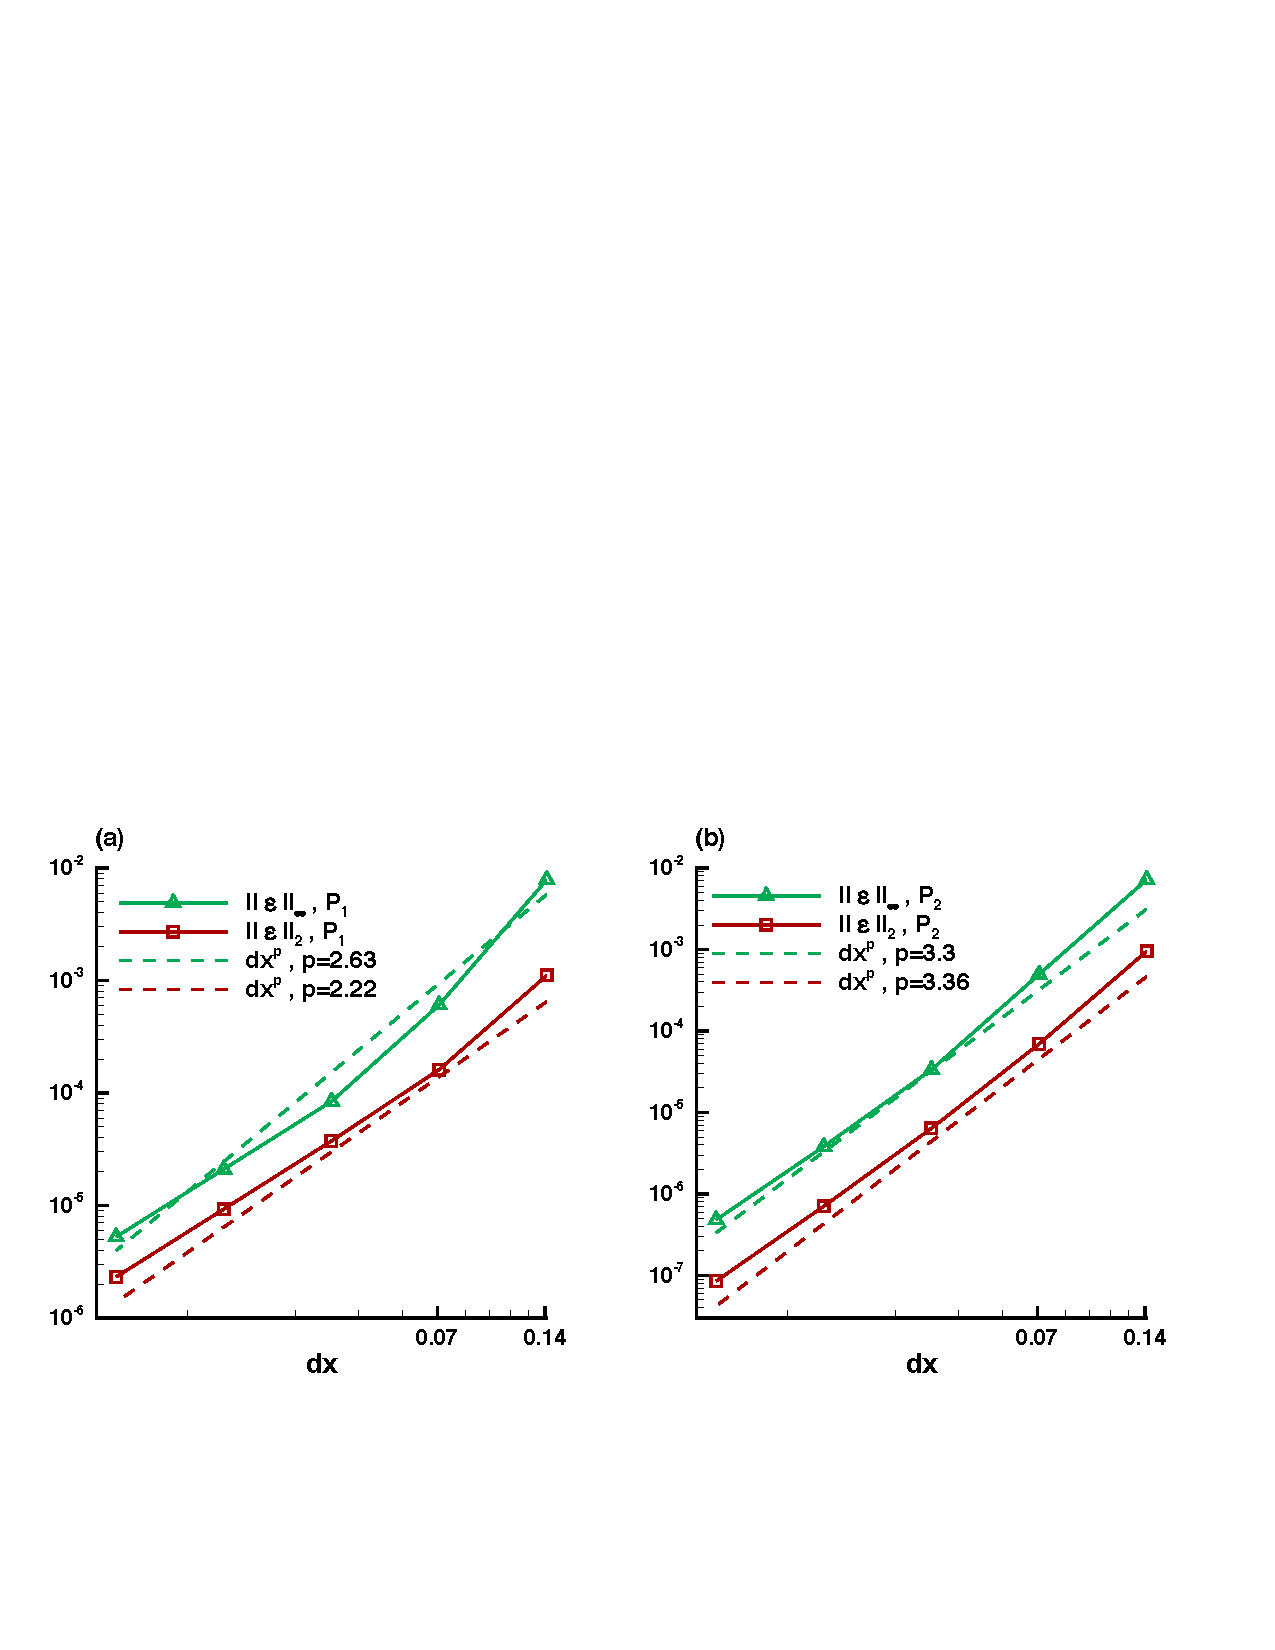
\includegraphics[width=0.98\textwidth]{Fig_cap_2/Convergence_BURGGRAF} 
	\end{center}
	\caption{Burggraf flow. Evolution of the global error $\| \varepsilon_h \|$ for both $\mathcal{L}_2$-norm and $\mathcal{L}_\infty$-norm, with different grid size. A Taylor-Hood finite element (P$_2$ for velocity and P$_1$ for pressure) is used for space discretization by taking either P$_1$ finite element (a) or P$_2$ finite element (b) for the temperature field.}
	\label{fig-conv-burggraf}
\end{figure}

To demonstrate the space accuracy of our method, we compute the well-known analytical solution called the Burggraf flow.
It consists of a steady recirculating flow in a square cavity $[ 0 , 1] \times [ 0 , 1]$, with a moving wall at the top boundary and non-slip wall conditions at the others :

\begin{eqnarray}
   u(x,0) &=& u(0,y) = u(1,y) = 0, \\
   u(x,1) &=& \sigma (x^4 - 2x^3 + x^2).
\end{eqnarray}
Besides, constant temperatures are imposed at the top and the bottom walls, while others are assumed to be adiabatic.
The exact solution of the flow is:
\begin{eqnarray}
   u1(x,y) &=& \sigma g'(x) h'(y), \\\nonumber
   u2(x,y) &=& - \sigma g''(x) h(y), \\\nonumber
   p(x,y)   &=& \frac{\sigma}{Re} \left( h^{(3)}(y) g(x) + g''(x)h'(y) \right) + \frac{\sigma}{2} g'(x)^2 \left( h(y)h''(y)-h'(y)^2 \right),\\ \nonumber
   T(x,y) &=& T_{c} + (T_{h} - T_{c}) y + a(x) b(y), \\ \nonumber
\end{eqnarray}
with,
\begin{eqnarray}
   g(x) &=& \frac{x^5}{5} - \frac{x^4}{2} - \frac{x^3}{3}, \\ \nonumber
   h(y) &=& y^4 - y^2, \\ \nonumber
   a(x) &=& \cos (\pi x), \\ \nonumber
   b(x) &=& y(1-y).
\end{eqnarray}
Hence, forcing term are defined as follows:

\begin{eqnarray}
   f_{u1} &=& 0 \\ \nonumber
   f_{u2} &=& \sigma^2 h(y) h'(y) \left( g''(x)^2 - g'(x)g^{(3)}(x) \right) \\ \nonumber
   &+& \frac{\sigma}{Re}\left( g^{(4)}(x) h(y) + 2 g''(x)h''(y) + g(x) h^{(4)}(y) \right) \\ \nonumber
   &+& \frac{\sigma^2}{2} g'(x)^2 \left( h(y) h^{(3)}(y) - h'(y)h''(y) \right) - \frac{Ra}{Pr Re^2} T(x,y),\\ \nonumber
   f_T &=& u1(x,y) a'(x) b(y) + u2(x,y) \left( T_h - T_c + a(x) b'(y) \right) \\ \nonumber
   &-& \frac{K}{Re Pr} \left( a''(x)b(y) + a(x) b''(y) \right).
\end{eqnarray}
We use the Taylor-Hood finite element (P$_2$ for velocity and P$_1$ for pressure) for the space discretization with either P$_1$ or P$_2$ finite element for the temperature field.
Figure \ref{fig-conv-burggraf} plots the decrease of the global discretization error $\| \varepsilon_h \|$ for both $\mathcal{L}_2$-norm and $\mathcal{L}_\infty$-norm function of the grid size.
The expected second order convergence is obtained with a P$_1$ finite element for the temperature (Figure \ref{fig-conv-burggraf}a), and even a nearly third order is noticed with a P$_2$ finite element on the temperature (Figure \ref{fig-conv-burggraf}b).

\subsubsection{Manufactured solution} \label{subsub-conv-nourg}
\begin{figure}
	\begin{center}
		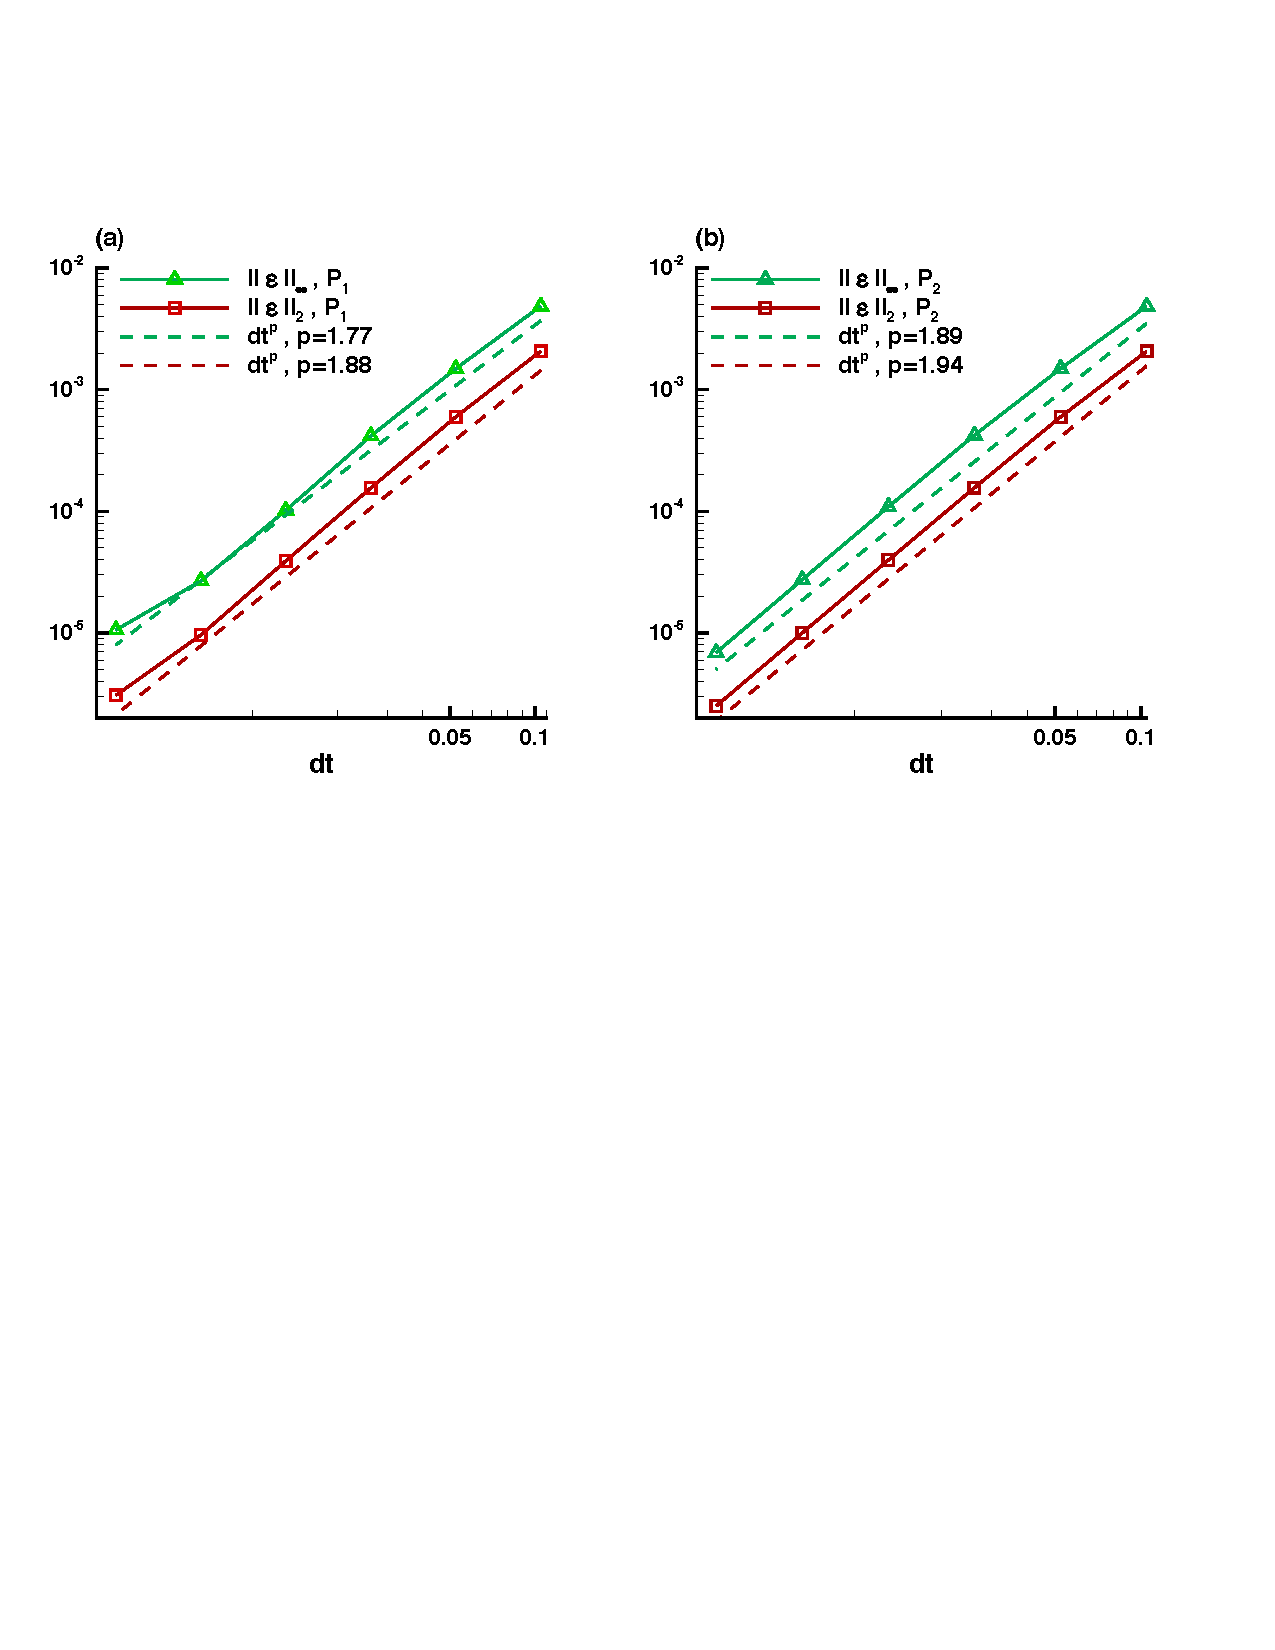
\includegraphics[width=0.98\textwidth]{Fig_cap_2/Convergence_BDF2} 
	\end{center}
	\caption{Manufactured solution of \cite{nourgaliev2016fully} for unsteady incompressible Navier-Stokes equation at dimensionless time $t = \pi$. Evolution of the global error $\| \varepsilon_h \|$ for both $\mathcal{L}_2$-norm and $\mathcal{L}_\infty$-norm, with different time steps, with a P$_1$ finite element (a) and a P$_2$ finite element (b) for the temperature.}
	\label{fig-conv-bdf2}
\end{figure}

The time integration is based on the implicit second order scheme BDF2.
We use the manufactured solution of \cite{nourgaliev2016fully} to measure the temporal convergence order.
\begin{eqnarray}
	u_1(x,y,t) &=& \left( \delta U_0 + \alpha_u \, \sin(t) \right) \, \cos(x+ \gamma_1 t) \, \sin(y+ \gamma_2 t), \\ \nonumber
	u_2(x,y,t) &=& - \left( \delta U_0 + \alpha_u \sin(t) \right) \, \sin(x+ \gamma_1 t) \, \cos(y+ \gamma_2 t), \\ \nonumber
	T(x,y,t) &=& \bar{T} + \left( \delta T_0 + \alpha_t \sin(t) \right) \, \cos(x+ \gamma_1 t) \, \sin(y+ \gamma_2 t), \\ \nonumber
	p(x,y,t) &=& \bar{P} + \left(\delta P_0 + \alpha_p \sin(t) \right) \, \sin(x+ \gamma_1 t) \, \cos(y+ \gamma_2 t), 
\end{eqnarray}
The value of the constants are reported on Table \ref{tab-constant}.
\begin{table}[!h]
\centering
\begin{tabular}{*{10}{c}}
 % \toprule
  $\gamma_1$ & $\gamma_2$ & $\bar{P}$ & $\bar{T}$ & $\delta P_0$ & $\delta T_0$ & $\delta U_0$ & $\alpha_p$ & $\alpha_u$ & $\alpha_t$\\
   \midrule
  $0.1$ & $0.1$ & $0$ & $1.0$ &  $0.1$ & $1.0$ & $1.0$ & $0.05$ & $0.4$ & $0.1$ \\
 % \bottomrule

 \end{tabular}
\caption{Parameter for the manufactured solution.}
\label{tab-constant}
\end{table}

\noindent Thus, forcing terms are:

\begin{eqnarray}
	f_x &=& \alpha_u \, \cos(t) \, \cos(a) \sin(b) - U_c \, \gamma_1 \, \sin(a) \sin(b) + U_c \, \gamma_2  \, \cos(a)\cos(b) \\ \nonumber
	  & & - U_c \,  u_1(x,y,t) \, \sin(a) \sin(b) + U_c \,  u_2(x,y,t) \, \cos(a) \cos(b)
	  + P_c \, \cos(a) \cos(b)\\ \nonumber
	  & & + \frac{1}{Re} \, u(x,y,t), \\	  \nonumber
	f_y &=& - \alpha_u \,  \cos(t)  \, \sin(a) \cos(b) - U_c \,  \gamma_1  \,  \cos(a) \cos(b) + U_c \,  \gamma_2 \,  \sin(a)\sin(b) \\ \nonumber
		  & & - U_c \,  u_1(x,y,t)  \,  \cos(a) \cos(b) + U_c  \, u_2(x,y,t)  \,  \sin(a) \sin(b)
		  -  P_c  \,  \sin(a)  \,  \sin(b)\\ \nonumber
		  & & -\frac{1}{Re} \,  v(x,y,t)
		  - \frac{Ra}{Pr Re^2} \,  T(x,y,t), \\  \nonumber
	f_{\theta} &=& \alpha_t \,  \cos(t) \,  \cos(a) \sin(b) -  T_c  \,  \gamma_1 \,  \sin(a) \sin(b) + T_c \,   \gamma_2  \,  \cos(a)\cos(b) \\ \nonumber
		  & &-  T_c \,  u_1(x,y,t)  \,  \sin(a) \sin(b)  
		  +   T_c  \,  u_2(x,y,t)  \, \cos(a) \cos(b) 
		  + \frac{K}{Re Pr} \,  T_c  \, \cos(a) \sin(b), \\ \nonumber
\end{eqnarray}

with: 
$	U_c = (\delta U_0 + \alpha_u \sin(t)), \,
	T_c = (\delta T_0 + \alpha_u \sin(t)), \,
	P_c = (\delta P_0 + \alpha_u \sin(t)), $ \\
and $	a = (x+ \gamma_1 t), \,
	b = (y+ \gamma_2 t). \\$

Since the space convergence rate was evaluated in \S \ref{subsub-conv-burg}, we fixe the grid size to $dx = 0.01$ to ensure a small spatial discretization errors, and we vary decreasingly the time step.
Time convergence is displayed in Figure \ref{fig-conv-bdf2}. 
The evolution of the global error with different time steps is plotted for both  $\mathcal{L}_2$-norm (red line) and $\mathcal{L}_\infty$-norm (green line), and the expected second order convergence is exposed for both P$_1$ (Figure \ref{fig-conv-bdf2}a) and P$_2$ (Figure \ref{fig-conv-bdf2}b) finite element for the temperature.



%\graphicspath{{\figpath/CARMAN-COZENY}}
%\include{chap01_CK_2017}
%\graphicspath{{\figpath/CARMAN-COZENY}}
%\include{chap02_CK_2017}
%\include{appendix}
%%%%%%%%%%%%%%%%%%%%%%%%%%%%%%%%%%%%%%%%%%%%%%%

%%%%%%%%=====================================================
%\part{Bibliography}
%\parttoc
%%%%%%%=====================================================
\addcontentsline{toc}{chapter}{Bibliography}

\bibliographystyle{\stypath/plainnat-io}
%\bibliographystyle{plain}
%\renewcommand{\bibname}{\em }
\bibliography{\bibpath/bib_thesis_2}
\end{document}
